% Created by tikzDevice version 0.12.6 on 2025-02-16 19:08:38
% !TEX encoding = UTF-8 Unicode
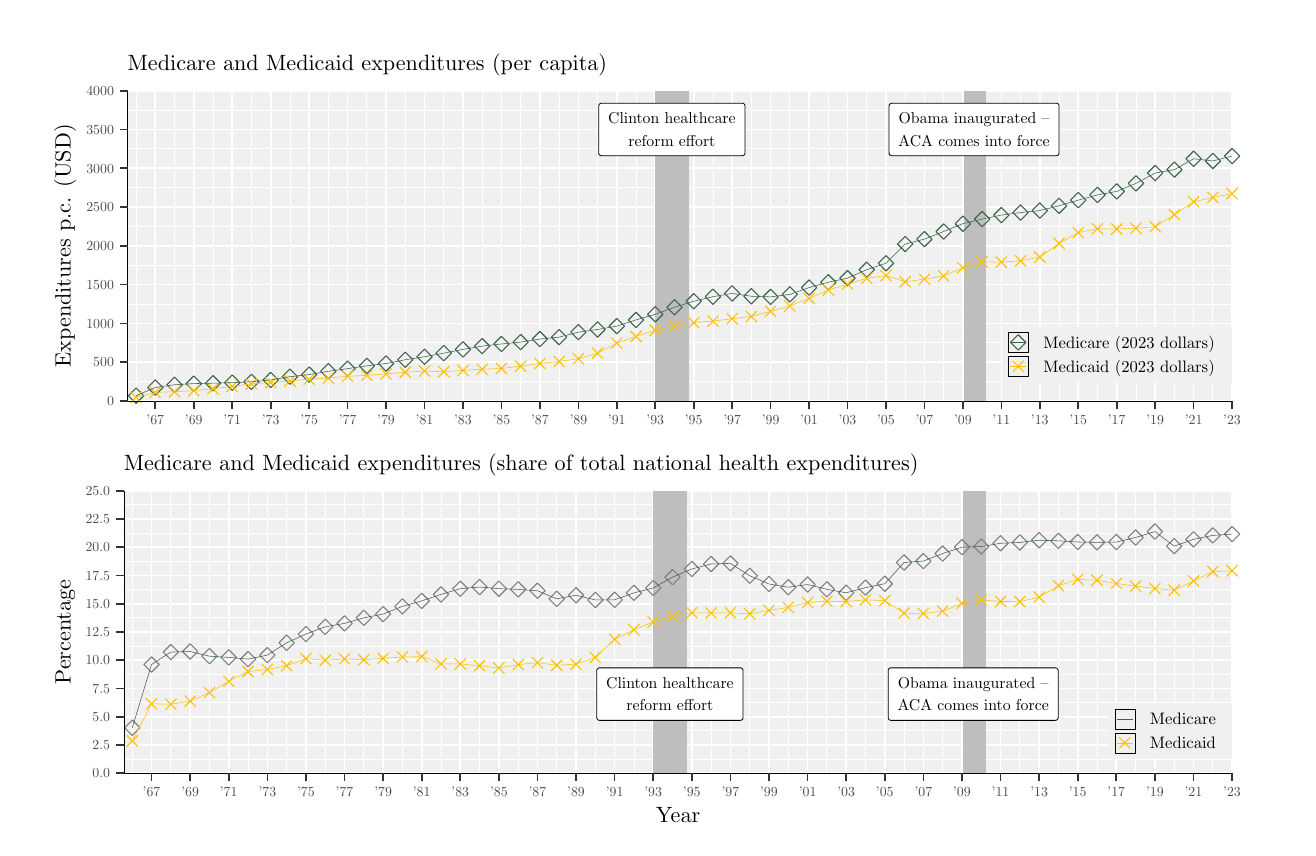
\begin{tikzpicture}[x=1pt,y=1pt]
\definecolor{fillColor}{RGB}{255,255,255}
\path[use as bounding box,fill=fillColor,fill opacity=0.00] (0,0) rectangle (455.30,289.08);
\begin{scope}
\path[clip] (  0.00,144.54) rectangle (455.30,289.08);
\definecolor{drawColor}{RGB}{255,255,255}
\definecolor{fillColor}{RGB}{255,255,255}

\path[draw=drawColor,line width= 0.6pt,line join=round,line cap=round,fill=fillColor] (  0.00,144.54) rectangle (455.30,289.08);
\end{scope}
\begin{scope}
\path[clip] (  0.00,  0.00) rectangle (455.30,289.08);
\definecolor{fillColor}{gray}{0.94}

\path[fill=fillColor] ( 36.14,154.20) rectangle (435.30,266.30);
\definecolor{drawColor}{RGB}{255,255,255}

\path[draw=drawColor,line width= 0.3pt,line join=round] ( 36.14,161.20) --
	(435.30,161.20);

\path[draw=drawColor,line width= 0.3pt,line join=round] ( 36.14,175.22) --
	(435.30,175.22);

\path[draw=drawColor,line width= 0.3pt,line join=round] ( 36.14,189.23) --
	(435.30,189.23);

\path[draw=drawColor,line width= 0.3pt,line join=round] ( 36.14,203.24) --
	(435.30,203.24);

\path[draw=drawColor,line width= 0.3pt,line join=round] ( 36.14,217.26) --
	(435.30,217.26);

\path[draw=drawColor,line width= 0.3pt,line join=round] ( 36.14,231.27) --
	(435.30,231.27);

\path[draw=drawColor,line width= 0.3pt,line join=round] ( 36.14,245.28) --
	(435.30,245.28);

\path[draw=drawColor,line width= 0.3pt,line join=round] ( 36.14,259.30) --
	(435.30,259.30);

\path[draw=drawColor,line width= 0.3pt,line join=round] ( 39.18,154.20) --
	( 39.18,266.30);

\path[draw=drawColor,line width= 0.3pt,line join=round] ( 53.08,154.20) --
	( 53.08,266.30);

\path[draw=drawColor,line width= 0.3pt,line join=round] ( 66.97,154.20) --
	( 66.97,266.30);

\path[draw=drawColor,line width= 0.3pt,line join=round] ( 80.87,154.20) --
	( 80.87,266.30);

\path[draw=drawColor,line width= 0.3pt,line join=round] ( 94.76,154.20) --
	( 94.76,266.30);

\path[draw=drawColor,line width= 0.3pt,line join=round] (108.66,154.20) --
	(108.66,266.30);

\path[draw=drawColor,line width= 0.3pt,line join=round] (122.56,154.20) --
	(122.56,266.30);

\path[draw=drawColor,line width= 0.3pt,line join=round] (136.45,154.20) --
	(136.45,266.30);

\path[draw=drawColor,line width= 0.3pt,line join=round] (150.35,154.20) --
	(150.35,266.30);

\path[draw=drawColor,line width= 0.3pt,line join=round] (164.24,154.20) --
	(164.24,266.30);

\path[draw=drawColor,line width= 0.3pt,line join=round] (178.14,154.20) --
	(178.14,266.30);

\path[draw=drawColor,line width= 0.3pt,line join=round] (192.03,154.20) --
	(192.03,266.30);

\path[draw=drawColor,line width= 0.3pt,line join=round] (205.93,154.20) --
	(205.93,266.30);

\path[draw=drawColor,line width= 0.3pt,line join=round] (219.83,154.20) --
	(219.83,266.30);

\path[draw=drawColor,line width= 0.3pt,line join=round] (233.72,154.20) --
	(233.72,266.30);

\path[draw=drawColor,line width= 0.3pt,line join=round] (247.62,154.20) --
	(247.62,266.30);

\path[draw=drawColor,line width= 0.3pt,line join=round] (261.51,154.20) --
	(261.51,266.30);

\path[draw=drawColor,line width= 0.3pt,line join=round] (275.41,154.20) --
	(275.41,266.30);

\path[draw=drawColor,line width= 0.3pt,line join=round] (289.31,154.20) --
	(289.31,266.30);

\path[draw=drawColor,line width= 0.3pt,line join=round] (303.20,154.20) --
	(303.20,266.30);

\path[draw=drawColor,line width= 0.3pt,line join=round] (317.10,154.20) --
	(317.10,266.30);

\path[draw=drawColor,line width= 0.3pt,line join=round] (330.99,154.20) --
	(330.99,266.30);

\path[draw=drawColor,line width= 0.3pt,line join=round] (344.89,154.20) --
	(344.89,266.30);

\path[draw=drawColor,line width= 0.3pt,line join=round] (358.78,154.20) --
	(358.78,266.30);

\path[draw=drawColor,line width= 0.3pt,line join=round] (372.68,154.20) --
	(372.68,266.30);

\path[draw=drawColor,line width= 0.3pt,line join=round] (386.58,154.20) --
	(386.58,266.30);

\path[draw=drawColor,line width= 0.3pt,line join=round] (400.47,154.20) --
	(400.47,266.30);

\path[draw=drawColor,line width= 0.3pt,line join=round] (414.37,154.20) --
	(414.37,266.30);

\path[draw=drawColor,line width= 0.3pt,line join=round] (428.26,154.20) --
	(428.26,266.30);

\path[draw=drawColor,line width= 0.6pt,line join=round] ( 36.14,154.20) --
	(435.30,154.20);

\path[draw=drawColor,line width= 0.6pt,line join=round] ( 36.14,168.21) --
	(435.30,168.21);

\path[draw=drawColor,line width= 0.6pt,line join=round] ( 36.14,182.22) --
	(435.30,182.22);

\path[draw=drawColor,line width= 0.6pt,line join=round] ( 36.14,196.24) --
	(435.30,196.24);

\path[draw=drawColor,line width= 0.6pt,line join=round] ( 36.14,210.25) --
	(435.30,210.25);

\path[draw=drawColor,line width= 0.6pt,line join=round] ( 36.14,224.26) --
	(435.30,224.26);

\path[draw=drawColor,line width= 0.6pt,line join=round] ( 36.14,238.28) --
	(435.30,238.28);

\path[draw=drawColor,line width= 0.6pt,line join=round] ( 36.14,252.29) --
	(435.30,252.29);

\path[draw=drawColor,line width= 0.6pt,line join=round] ( 36.14,266.30) --
	(435.30,266.30);

\path[draw=drawColor,line width= 0.6pt,line join=round] ( 46.12,154.20) --
	( 46.12,266.30);

\path[draw=drawColor,line width= 0.6pt,line join=round] ( 60.03,154.20) --
	( 60.03,266.30);

\path[draw=drawColor,line width= 0.6pt,line join=round] ( 73.92,154.20) --
	( 73.92,266.30);

\path[draw=drawColor,line width= 0.6pt,line join=round] ( 87.82,154.20) --
	( 87.82,266.30);

\path[draw=drawColor,line width= 0.6pt,line join=round] (101.71,154.20) --
	(101.71,266.30);

\path[draw=drawColor,line width= 0.6pt,line join=round] (115.61,154.20) --
	(115.61,266.30);

\path[draw=drawColor,line width= 0.6pt,line join=round] (129.50,154.20) --
	(129.50,266.30);

\path[draw=drawColor,line width= 0.6pt,line join=round] (143.40,154.20) --
	(143.40,266.30);

\path[draw=drawColor,line width= 0.6pt,line join=round] (157.29,154.20) --
	(157.29,266.30);

\path[draw=drawColor,line width= 0.6pt,line join=round] (171.20,154.20) --
	(171.20,266.30);

\path[draw=drawColor,line width= 0.6pt,line join=round] (185.08,154.20) --
	(185.08,266.30);

\path[draw=drawColor,line width= 0.6pt,line join=round] (198.99,154.20) --
	(198.99,266.30);

\path[draw=drawColor,line width= 0.6pt,line join=round] (212.87,154.20) --
	(212.87,266.30);

\path[draw=drawColor,line width= 0.6pt,line join=round] (226.78,154.20) --
	(226.78,266.30);

\path[draw=drawColor,line width= 0.6pt,line join=round] (240.67,154.20) --
	(240.67,266.30);

\path[draw=drawColor,line width= 0.6pt,line join=round] (254.57,154.20) --
	(254.57,266.30);

\path[draw=drawColor,line width= 0.6pt,line join=round] (268.46,154.20) --
	(268.46,266.30);

\path[draw=drawColor,line width= 0.6pt,line join=round] (282.36,154.20) --
	(282.36,266.30);

\path[draw=drawColor,line width= 0.6pt,line join=round] (296.25,154.20) --
	(296.25,266.30);

\path[draw=drawColor,line width= 0.6pt,line join=round] (310.15,154.20) --
	(310.15,266.30);

\path[draw=drawColor,line width= 0.6pt,line join=round] (324.04,154.20) --
	(324.04,266.30);

\path[draw=drawColor,line width= 0.6pt,line join=round] (337.95,154.20) --
	(337.95,266.30);

\path[draw=drawColor,line width= 0.6pt,line join=round] (351.83,154.20) --
	(351.83,266.30);

\path[draw=drawColor,line width= 0.6pt,line join=round] (365.74,154.20) --
	(365.74,266.30);

\path[draw=drawColor,line width= 0.6pt,line join=round] (379.62,154.20) --
	(379.62,266.30);

\path[draw=drawColor,line width= 0.6pt,line join=round] (393.53,154.20) --
	(393.53,266.30);

\path[draw=drawColor,line width= 0.6pt,line join=round] (407.41,154.20) --
	(407.41,266.30);

\path[draw=drawColor,line width= 0.6pt,line join=round] (421.32,154.20) --
	(421.32,266.30);

\path[draw=drawColor,line width= 0.6pt,line join=round] (435.21,154.20) --
	(435.21,266.30);
\definecolor{fillColor}{RGB}{190,190,190}

\path[fill=fillColor,fill opacity=0.01] (226.78,154.20) rectangle (238.82,266.30);

\path[fill=fillColor,fill opacity=0.01] (226.78,154.20) rectangle (238.82,266.30);

\path[fill=fillColor,fill opacity=0.01] (226.78,154.20) rectangle (238.82,266.30);

\path[fill=fillColor,fill opacity=0.01] (226.78,154.20) rectangle (238.82,266.30);

\path[fill=fillColor,fill opacity=0.01] (226.78,154.20) rectangle (238.82,266.30);

\path[fill=fillColor,fill opacity=0.01] (226.78,154.20) rectangle (238.82,266.30);

\path[fill=fillColor,fill opacity=0.01] (226.78,154.20) rectangle (238.82,266.30);

\path[fill=fillColor,fill opacity=0.01] (226.78,154.20) rectangle (238.82,266.30);

\path[fill=fillColor,fill opacity=0.01] (226.78,154.20) rectangle (238.82,266.30);

\path[fill=fillColor,fill opacity=0.01] (226.78,154.20) rectangle (238.82,266.30);

\path[fill=fillColor,fill opacity=0.01] (226.78,154.20) rectangle (238.82,266.30);

\path[fill=fillColor,fill opacity=0.01] (226.78,154.20) rectangle (238.82,266.30);

\path[fill=fillColor,fill opacity=0.01] (226.78,154.20) rectangle (238.82,266.30);

\path[fill=fillColor,fill opacity=0.01] (226.78,154.20) rectangle (238.82,266.30);

\path[fill=fillColor,fill opacity=0.01] (226.78,154.20) rectangle (238.82,266.30);

\path[fill=fillColor,fill opacity=0.01] (226.78,154.20) rectangle (238.82,266.30);

\path[fill=fillColor,fill opacity=0.01] (226.78,154.20) rectangle (238.82,266.30);

\path[fill=fillColor,fill opacity=0.01] (226.78,154.20) rectangle (238.82,266.30);

\path[fill=fillColor,fill opacity=0.01] (226.78,154.20) rectangle (238.82,266.30);

\path[fill=fillColor,fill opacity=0.01] (226.78,154.20) rectangle (238.82,266.30);

\path[fill=fillColor,fill opacity=0.01] (226.78,154.20) rectangle (238.82,266.30);

\path[fill=fillColor,fill opacity=0.01] (226.78,154.20) rectangle (238.82,266.30);

\path[fill=fillColor,fill opacity=0.01] (226.78,154.20) rectangle (238.82,266.30);

\path[fill=fillColor,fill opacity=0.01] (226.78,154.20) rectangle (238.82,266.30);

\path[fill=fillColor,fill opacity=0.01] (226.78,154.20) rectangle (238.82,266.30);

\path[fill=fillColor,fill opacity=0.01] (226.78,154.20) rectangle (238.82,266.30);

\path[fill=fillColor,fill opacity=0.01] (226.78,154.20) rectangle (238.82,266.30);

\path[fill=fillColor,fill opacity=0.01] (226.78,154.20) rectangle (238.82,266.30);

\path[fill=fillColor,fill opacity=0.01] (226.78,154.20) rectangle (238.82,266.30);

\path[fill=fillColor,fill opacity=0.01] (226.78,154.20) rectangle (238.82,266.30);

\path[fill=fillColor,fill opacity=0.01] (226.78,154.20) rectangle (238.82,266.30);

\path[fill=fillColor,fill opacity=0.01] (226.78,154.20) rectangle (238.82,266.30);

\path[fill=fillColor,fill opacity=0.01] (226.78,154.20) rectangle (238.82,266.30);

\path[fill=fillColor,fill opacity=0.01] (226.78,154.20) rectangle (238.82,266.30);

\path[fill=fillColor,fill opacity=0.01] (226.78,154.20) rectangle (238.82,266.30);

\path[fill=fillColor,fill opacity=0.01] (226.78,154.20) rectangle (238.82,266.30);

\path[fill=fillColor,fill opacity=0.01] (226.78,154.20) rectangle (238.82,266.30);

\path[fill=fillColor,fill opacity=0.01] (226.78,154.20) rectangle (238.82,266.30);

\path[fill=fillColor,fill opacity=0.01] (226.78,154.20) rectangle (238.82,266.30);

\path[fill=fillColor,fill opacity=0.01] (226.78,154.20) rectangle (238.82,266.30);

\path[fill=fillColor,fill opacity=0.01] (226.78,154.20) rectangle (238.82,266.30);

\path[fill=fillColor,fill opacity=0.01] (226.78,154.20) rectangle (238.82,266.30);

\path[fill=fillColor,fill opacity=0.01] (226.78,154.20) rectangle (238.82,266.30);

\path[fill=fillColor,fill opacity=0.01] (226.78,154.20) rectangle (238.82,266.30);

\path[fill=fillColor,fill opacity=0.01] (226.78,154.20) rectangle (238.82,266.30);

\path[fill=fillColor,fill opacity=0.01] (226.78,154.20) rectangle (238.82,266.30);

\path[fill=fillColor,fill opacity=0.01] (226.78,154.20) rectangle (238.82,266.30);

\path[fill=fillColor,fill opacity=0.01] (226.78,154.20) rectangle (238.82,266.30);

\path[fill=fillColor,fill opacity=0.01] (226.78,154.20) rectangle (238.82,266.30);

\path[fill=fillColor,fill opacity=0.01] (226.78,154.20) rectangle (238.82,266.30);

\path[fill=fillColor,fill opacity=0.01] (226.78,154.20) rectangle (238.82,266.30);

\path[fill=fillColor,fill opacity=0.01] (226.78,154.20) rectangle (238.82,266.30);

\path[fill=fillColor,fill opacity=0.01] (226.78,154.20) rectangle (238.82,266.30);

\path[fill=fillColor,fill opacity=0.01] (226.78,154.20) rectangle (238.82,266.30);

\path[fill=fillColor,fill opacity=0.01] (226.78,154.20) rectangle (238.82,266.30);

\path[fill=fillColor,fill opacity=0.01] (226.78,154.20) rectangle (238.82,266.30);

\path[fill=fillColor,fill opacity=0.01] (226.78,154.20) rectangle (238.82,266.30);

\path[fill=fillColor,fill opacity=0.01] (226.78,154.20) rectangle (238.82,266.30);

\path[fill=fillColor,fill opacity=0.01] (226.78,154.20) rectangle (238.82,266.30);

\path[fill=fillColor,fill opacity=0.01] (226.78,154.20) rectangle (238.82,266.30);

\path[fill=fillColor,fill opacity=0.01] (226.78,154.20) rectangle (238.82,266.30);

\path[fill=fillColor,fill opacity=0.01] (226.78,154.20) rectangle (238.82,266.30);

\path[fill=fillColor,fill opacity=0.01] (226.78,154.20) rectangle (238.82,266.30);

\path[fill=fillColor,fill opacity=0.01] (226.78,154.20) rectangle (238.82,266.30);

\path[fill=fillColor,fill opacity=0.01] (338.31,154.20) rectangle (346.43,266.30);

\path[fill=fillColor,fill opacity=0.01] (338.31,154.20) rectangle (346.43,266.30);

\path[fill=fillColor,fill opacity=0.01] (338.31,154.20) rectangle (346.43,266.30);

\path[fill=fillColor,fill opacity=0.01] (338.31,154.20) rectangle (346.43,266.30);

\path[fill=fillColor,fill opacity=0.01] (338.31,154.20) rectangle (346.43,266.30);

\path[fill=fillColor,fill opacity=0.01] (338.31,154.20) rectangle (346.43,266.30);

\path[fill=fillColor,fill opacity=0.01] (338.31,154.20) rectangle (346.43,266.30);

\path[fill=fillColor,fill opacity=0.01] (338.31,154.20) rectangle (346.43,266.30);

\path[fill=fillColor,fill opacity=0.01] (338.31,154.20) rectangle (346.43,266.30);

\path[fill=fillColor,fill opacity=0.01] (338.31,154.20) rectangle (346.43,266.30);

\path[fill=fillColor,fill opacity=0.01] (338.31,154.20) rectangle (346.43,266.30);

\path[fill=fillColor,fill opacity=0.01] (338.31,154.20) rectangle (346.43,266.30);

\path[fill=fillColor,fill opacity=0.01] (338.31,154.20) rectangle (346.43,266.30);

\path[fill=fillColor,fill opacity=0.01] (338.31,154.20) rectangle (346.43,266.30);

\path[fill=fillColor,fill opacity=0.01] (338.31,154.20) rectangle (346.43,266.30);

\path[fill=fillColor,fill opacity=0.01] (338.31,154.20) rectangle (346.43,266.30);

\path[fill=fillColor,fill opacity=0.01] (338.31,154.20) rectangle (346.43,266.30);

\path[fill=fillColor,fill opacity=0.01] (338.31,154.20) rectangle (346.43,266.30);

\path[fill=fillColor,fill opacity=0.01] (338.31,154.20) rectangle (346.43,266.30);

\path[fill=fillColor,fill opacity=0.01] (338.31,154.20) rectangle (346.43,266.30);

\path[fill=fillColor,fill opacity=0.01] (338.31,154.20) rectangle (346.43,266.30);

\path[fill=fillColor,fill opacity=0.01] (338.31,154.20) rectangle (346.43,266.30);

\path[fill=fillColor,fill opacity=0.01] (338.31,154.20) rectangle (346.43,266.30);

\path[fill=fillColor,fill opacity=0.01] (338.31,154.20) rectangle (346.43,266.30);

\path[fill=fillColor,fill opacity=0.01] (338.31,154.20) rectangle (346.43,266.30);

\path[fill=fillColor,fill opacity=0.01] (338.31,154.20) rectangle (346.43,266.30);

\path[fill=fillColor,fill opacity=0.01] (338.31,154.20) rectangle (346.43,266.30);

\path[fill=fillColor,fill opacity=0.01] (338.31,154.20) rectangle (346.43,266.30);

\path[fill=fillColor,fill opacity=0.01] (338.31,154.20) rectangle (346.43,266.30);

\path[fill=fillColor,fill opacity=0.01] (338.31,154.20) rectangle (346.43,266.30);

\path[fill=fillColor,fill opacity=0.01] (338.31,154.20) rectangle (346.43,266.30);

\path[fill=fillColor,fill opacity=0.01] (338.31,154.20) rectangle (346.43,266.30);

\path[fill=fillColor,fill opacity=0.01] (338.31,154.20) rectangle (346.43,266.30);

\path[fill=fillColor,fill opacity=0.01] (338.31,154.20) rectangle (346.43,266.30);

\path[fill=fillColor,fill opacity=0.01] (338.31,154.20) rectangle (346.43,266.30);

\path[fill=fillColor,fill opacity=0.01] (338.31,154.20) rectangle (346.43,266.30);

\path[fill=fillColor,fill opacity=0.01] (338.31,154.20) rectangle (346.43,266.30);

\path[fill=fillColor,fill opacity=0.01] (338.31,154.20) rectangle (346.43,266.30);

\path[fill=fillColor,fill opacity=0.01] (338.31,154.20) rectangle (346.43,266.30);

\path[fill=fillColor,fill opacity=0.01] (338.31,154.20) rectangle (346.43,266.30);

\path[fill=fillColor,fill opacity=0.01] (338.31,154.20) rectangle (346.43,266.30);

\path[fill=fillColor,fill opacity=0.01] (338.31,154.20) rectangle (346.43,266.30);

\path[fill=fillColor,fill opacity=0.01] (338.31,154.20) rectangle (346.43,266.30);

\path[fill=fillColor,fill opacity=0.01] (338.31,154.20) rectangle (346.43,266.30);

\path[fill=fillColor,fill opacity=0.01] (338.31,154.20) rectangle (346.43,266.30);

\path[fill=fillColor,fill opacity=0.01] (338.31,154.20) rectangle (346.43,266.30);

\path[fill=fillColor,fill opacity=0.01] (338.31,154.20) rectangle (346.43,266.30);

\path[fill=fillColor,fill opacity=0.01] (338.31,154.20) rectangle (346.43,266.30);

\path[fill=fillColor,fill opacity=0.01] (338.31,154.20) rectangle (346.43,266.30);

\path[fill=fillColor,fill opacity=0.01] (338.31,154.20) rectangle (346.43,266.30);

\path[fill=fillColor,fill opacity=0.01] (338.31,154.20) rectangle (346.43,266.30);

\path[fill=fillColor,fill opacity=0.01] (338.31,154.20) rectangle (346.43,266.30);

\path[fill=fillColor,fill opacity=0.01] (338.31,154.20) rectangle (346.43,266.30);

\path[fill=fillColor,fill opacity=0.01] (338.31,154.20) rectangle (346.43,266.30);

\path[fill=fillColor,fill opacity=0.01] (338.31,154.20) rectangle (346.43,266.30);

\path[fill=fillColor,fill opacity=0.01] (338.31,154.20) rectangle (346.43,266.30);

\path[fill=fillColor,fill opacity=0.01] (338.31,154.20) rectangle (346.43,266.30);

\path[fill=fillColor,fill opacity=0.01] (338.31,154.20) rectangle (346.43,266.30);

\path[fill=fillColor,fill opacity=0.01] (338.31,154.20) rectangle (346.43,266.30);

\path[fill=fillColor,fill opacity=0.01] (338.31,154.20) rectangle (346.43,266.30);

\path[fill=fillColor,fill opacity=0.01] (338.31,154.20) rectangle (346.43,266.30);

\path[fill=fillColor,fill opacity=0.01] (338.31,154.20) rectangle (346.43,266.30);

\path[fill=fillColor,fill opacity=0.01] (338.31,154.20) rectangle (346.43,266.30);

\path[fill=fillColor,fill opacity=0.01] (338.31,154.20) rectangle (346.43,266.30);
\definecolor{drawColor}{RGB}{0,0,0}
\definecolor{fillColor}{RGB}{255,255,255}

\path[draw=drawColor,line width= 0.3pt,line join=round,line cap=round,fill=fillColor] (207.39,242.81) --
	(258.19,242.81) --
	(258.15,242.81) --
	(258.32,242.81) --
	(258.48,242.85) --
	(258.63,242.91) --
	(258.78,242.99) --
	(258.91,243.09) --
	(259.01,243.22) --
	(259.10,243.36) --
	(259.17,243.51) --
	(259.21,243.67) --
	(259.22,243.83) --
	(259.22,243.83) --
	(259.22,260.75) --
	(259.22,260.75) --
	(259.21,260.91) --
	(259.17,261.07) --
	(259.10,261.22) --
	(259.01,261.36) --
	(258.91,261.49) --
	(258.78,261.59) --
	(258.63,261.68) --
	(258.48,261.73) --
	(258.32,261.77) --
	(258.19,261.77) --
	(207.39,261.77) --
	(207.51,261.77) --
	(207.35,261.77) --
	(207.18,261.75) --
	(207.02,261.71) --
	(206.87,261.64) --
	(206.74,261.54) --
	(206.62,261.43) --
	(206.52,261.30) --
	(206.44,261.15) --
	(206.39,260.99) --
	(206.36,260.83) --
	(206.36,260.75) --
	(206.36,243.83) --
	(206.36,243.92) --
	(206.36,243.75) --
	(206.39,243.59) --
	(206.44,243.43) --
	(206.52,243.28) --
	(206.62,243.15) --
	(206.74,243.04) --
	(206.87,242.94) --
	(207.02,242.87) --
	(207.18,242.83) --
	(207.35,242.81) --
	cycle;
\end{scope}
\begin{scope}
\path[clip] (  0.00,  0.00) rectangle (455.30,289.08);
\definecolor{drawColor}{RGB}{0,0,0}

\node[text=drawColor,anchor=base,inner sep=0pt, outer sep=0pt, scale=  0.57] at (232.79,254.43) {Clinton healthcare };

\node[text=drawColor,anchor=base,inner sep=0pt, outer sep=0pt, scale=  0.57] at (232.79,246.23) { reform effort};
\end{scope}
\begin{scope}
\path[clip] (  0.00,  0.00) rectangle (455.30,289.08);
\definecolor{drawColor}{RGB}{0,0,0}
\definecolor{fillColor}{RGB}{255,255,255}

\path[draw=drawColor,line width= 0.3pt,line join=round,line cap=round,fill=fillColor] (312.29,242.81) --
	(371.66,242.81) --
	(371.62,242.81) --
	(371.79,242.81) --
	(371.95,242.85) --
	(372.10,242.91) --
	(372.25,242.99) --
	(372.38,243.09) --
	(372.49,243.22) --
	(372.57,243.36) --
	(372.64,243.51) --
	(372.68,243.67) --
	(372.69,243.83) --
	(372.69,243.83) --
	(372.69,260.75) --
	(372.69,260.75) --
	(372.68,260.91) --
	(372.64,261.07) --
	(372.57,261.22) --
	(372.49,261.36) --
	(372.38,261.49) --
	(372.25,261.59) --
	(372.10,261.68) --
	(371.95,261.73) --
	(371.79,261.77) --
	(371.66,261.77) --
	(312.29,261.77) --
	(312.42,261.77) --
	(312.25,261.77) --
	(312.09,261.75) --
	(311.93,261.71) --
	(311.78,261.64) --
	(311.64,261.54) --
	(311.52,261.43) --
	(311.42,261.30) --
	(311.35,261.15) --
	(311.29,260.99) --
	(311.27,260.83) --
	(311.26,260.75) --
	(311.26,243.83) --
	(311.27,243.92) --
	(311.27,243.75) --
	(311.29,243.59) --
	(311.35,243.43) --
	(311.42,243.28) --
	(311.52,243.15) --
	(311.64,243.04) --
	(311.78,242.94) --
	(311.93,242.87) --
	(312.09,242.83) --
	(312.25,242.81) --
	cycle;
\end{scope}
\begin{scope}
\path[clip] (  0.00,  0.00) rectangle (455.30,289.08);
\definecolor{drawColor}{RGB}{0,0,0}

\node[text=drawColor,anchor=base,inner sep=0pt, outer sep=0pt, scale=  0.57] at (341.98,254.43) {Obama inaugurated -- };

\node[text=drawColor,anchor=base,inner sep=0pt, outer sep=0pt, scale=  0.57] at (341.98,246.23) { ACA comes into force};
\end{scope}
\begin{scope}
\path[clip] (  0.00,  0.00) rectangle (455.30,289.08);
\definecolor{drawColor}{RGB}{60,100,75}

\path[draw=drawColor,line width= 0.4pt,line join=round,line cap=round] ( 36.41,156.08) --
	( 39.18,158.86) --
	( 41.96,156.08) --
	( 39.18,153.31) --
	cycle;

\path[draw=drawColor,line width= 0.4pt,line join=round,line cap=round] ( 43.35,159.04) --
	( 46.12,161.82) --
	( 48.90,159.04) --
	( 46.12,156.27) --
	cycle;

\path[draw=drawColor,line width= 0.4pt,line join=round,line cap=round] ( 50.29,160.04) --
	( 53.07,162.81) --
	( 55.84,160.04) --
	( 53.07,157.26) --
	cycle;

\path[draw=drawColor,line width= 0.4pt,line join=round,line cap=round] ( 57.26,160.47) --
	( 60.03,163.24) --
	( 62.80,160.47) --
	( 60.03,157.69) --
	cycle;

\path[draw=drawColor,line width= 0.4pt,line join=round,line cap=round] ( 64.20,160.61) --
	( 66.97,163.38) --
	( 69.75,160.61) --
	( 66.97,157.83) --
	cycle;

\path[draw=drawColor,line width= 0.4pt,line join=round,line cap=round] ( 71.14,160.81) --
	( 73.92,163.59) --
	( 76.69,160.81) --
	( 73.92,158.04) --
	cycle;

\path[draw=drawColor,line width= 0.4pt,line join=round,line cap=round] ( 78.08,161.11) --
	( 80.86,163.88) --
	( 83.63,161.11) --
	( 80.86,158.33) --
	cycle;

\path[draw=drawColor,line width= 0.4pt,line join=round,line cap=round] ( 85.05,161.77) --
	( 87.82,164.54) --
	( 90.60,161.77) --
	( 87.82,158.99) --
	cycle;

\path[draw=drawColor,line width= 0.4pt,line join=round,line cap=round] ( 91.99,162.96) --
	( 94.76,165.74) --
	( 97.54,162.96) --
	( 94.76,160.19) --
	cycle;

\path[draw=drawColor,line width= 0.4pt,line join=round,line cap=round] ( 98.93,163.72) --
	(101.71,166.50) --
	(104.48,163.72) --
	(101.71,160.95) --
	cycle;

\path[draw=drawColor,line width= 0.4pt,line join=round,line cap=round] (105.88,164.92) --
	(108.65,167.70) --
	(111.43,164.92) --
	(108.65,162.15) --
	cycle;

\path[draw=drawColor,line width= 0.4pt,line join=round,line cap=round] (112.84,165.87) --
	(115.61,168.65) --
	(118.39,165.87) --
	(115.61,163.10) --
	cycle;

\path[draw=drawColor,line width= 0.4pt,line join=round,line cap=round] (119.78,166.87) --
	(122.56,169.64) --
	(125.33,166.87) --
	(122.56,164.09) --
	cycle;

\path[draw=drawColor,line width= 0.4pt,line join=round,line cap=round] (126.72,167.72) --
	(129.50,170.49) --
	(132.27,167.72) --
	(129.50,164.94) --
	cycle;

\path[draw=drawColor,line width= 0.4pt,line join=round,line cap=round] (133.67,169.08) --
	(136.44,171.86) --
	(139.22,169.08) --
	(136.44,166.31) --
	cycle;

\path[draw=drawColor,line width= 0.4pt,line join=round,line cap=round] (140.63,170.16) --
	(143.40,172.94) --
	(146.18,170.16) --
	(143.40,167.39) --
	cycle;

\path[draw=drawColor,line width= 0.4pt,line join=round,line cap=round] (147.57,171.47) --
	(150.35,174.25) --
	(153.12,171.47) --
	(150.35,168.70) --
	cycle;

\path[draw=drawColor,line width= 0.4pt,line join=round,line cap=round] (154.52,172.83) --
	(157.29,175.60) --
	(160.07,172.83) --
	(157.29,170.05) --
	cycle;

\path[draw=drawColor,line width= 0.4pt,line join=round,line cap=round] (161.46,174.02) --
	(164.23,176.79) --
	(167.01,174.02) --
	(164.23,171.24) --
	cycle;

\path[draw=drawColor,line width= 0.4pt,line join=round,line cap=round] (168.42,174.79) --
	(171.20,177.57) --
	(173.97,174.79) --
	(171.20,172.02) --
	cycle;

\path[draw=drawColor,line width= 0.4pt,line join=round,line cap=round] (175.36,175.46) --
	(178.14,178.24) --
	(180.91,175.46) --
	(178.14,172.69) --
	cycle;

\path[draw=drawColor,line width= 0.4pt,line join=round,line cap=round] (182.31,176.56) --
	(185.08,179.34) --
	(187.86,176.56) --
	(185.08,173.79) --
	cycle;

\path[draw=drawColor,line width= 0.4pt,line join=round,line cap=round] (189.25,177.25) --
	(192.03,180.02) --
	(194.80,177.25) --
	(192.03,174.47) --
	cycle;

\path[draw=drawColor,line width= 0.4pt,line join=round,line cap=round] (196.21,179.06) --
	(198.99,181.83) --
	(201.76,179.06) --
	(198.99,176.28) --
	cycle;

\path[draw=drawColor,line width= 0.4pt,line join=round,line cap=round] (203.16,180.02) --
	(205.93,182.80) --
	(208.71,180.02) --
	(205.93,177.25) --
	cycle;

\path[draw=drawColor,line width= 0.4pt,line join=round,line cap=round] (210.10,181.23) --
	(212.87,184.01) --
	(215.65,181.23) --
	(212.87,178.46) --
	cycle;

\path[draw=drawColor,line width= 0.4pt,line join=round,line cap=round] (217.04,183.48) --
	(219.82,186.25) --
	(222.59,183.48) --
	(219.82,180.70) --
	cycle;

\path[draw=drawColor,line width= 0.4pt,line join=round,line cap=round] (224.00,185.50) --
	(226.78,188.28) --
	(229.55,185.50) --
	(226.78,182.73) --
	cycle;

\path[draw=drawColor,line width= 0.4pt,line join=round,line cap=round] (230.95,188.05) --
	(233.72,190.82) --
	(236.50,188.05) --
	(233.72,185.27) --
	cycle;

\path[draw=drawColor,line width= 0.4pt,line join=round,line cap=round] (237.89,190.23) --
	(240.67,193.00) --
	(243.44,190.23) --
	(240.67,187.45) --
	cycle;

\path[draw=drawColor,line width= 0.4pt,line join=round,line cap=round] (244.83,191.87) --
	(247.61,194.64) --
	(250.38,191.87) --
	(247.61,189.09) --
	cycle;

\path[draw=drawColor,line width= 0.4pt,line join=round,line cap=round] (251.80,193.05) --
	(254.57,195.82) --
	(257.35,193.05) --
	(254.57,190.27) --
	cycle;

\path[draw=drawColor,line width= 0.4pt,line join=round,line cap=round] (258.74,192.03) --
	(261.51,194.80) --
	(264.29,192.03) --
	(261.51,189.25) --
	cycle;

\path[draw=drawColor,line width= 0.4pt,line join=round,line cap=round] (265.68,191.81) --
	(268.46,194.59) --
	(271.23,191.81) --
	(268.46,189.04) --
	cycle;

\path[draw=drawColor,line width= 0.4pt,line join=round,line cap=round] (272.63,192.69) --
	(275.40,195.47) --
	(278.17,192.69) --
	(275.40,189.92) --
	cycle;

\path[draw=drawColor,line width= 0.4pt,line join=round,line cap=round] (279.59,195.16) --
	(282.36,197.94) --
	(285.14,195.16) --
	(282.36,192.39) --
	cycle;

\path[draw=drawColor,line width= 0.4pt,line join=round,line cap=round] (286.53,197.09) --
	(289.31,199.86) --
	(292.08,197.09) --
	(289.31,194.31) --
	cycle;

\path[draw=drawColor,line width= 0.4pt,line join=round,line cap=round] (293.47,198.56) --
	(296.25,201.33) --
	(299.02,198.56) --
	(296.25,195.78) --
	cycle;

\path[draw=drawColor,line width= 0.4pt,line join=round,line cap=round] (300.42,201.62) --
	(303.19,204.39) --
	(305.97,201.62) --
	(303.19,198.84) --
	cycle;

\path[draw=drawColor,line width= 0.4pt,line join=round,line cap=round] (307.38,203.94) --
	(310.15,206.71) --
	(312.93,203.94) --
	(310.15,201.16) --
	cycle;

\path[draw=drawColor,line width= 0.4pt,line join=round,line cap=round] (314.32,210.89) --
	(317.10,213.66) --
	(319.87,210.89) --
	(317.10,208.11) --
	cycle;

\path[draw=drawColor,line width= 0.4pt,line join=round,line cap=round] (321.26,212.66) --
	(324.04,215.44) --
	(326.81,212.66) --
	(324.04,209.89) --
	cycle;

\path[draw=drawColor,line width= 0.4pt,line join=round,line cap=round] (328.21,215.42) --
	(330.98,218.19) --
	(333.76,215.42) --
	(330.98,212.64) --
	cycle;

\path[draw=drawColor,line width= 0.4pt,line join=round,line cap=round] (335.17,218.24) --
	(337.95,221.01) --
	(340.72,218.24) --
	(337.95,215.46) --
	cycle;

\path[draw=drawColor,line width= 0.4pt,line join=round,line cap=round] (342.11,219.91) --
	(344.89,222.69) --
	(347.66,219.91) --
	(344.89,217.14) --
	cycle;

\path[draw=drawColor,line width= 0.4pt,line join=round,line cap=round] (349.06,221.36) --
	(351.83,224.13) --
	(354.61,221.36) --
	(351.83,218.58) --
	cycle;

\path[draw=drawColor,line width= 0.4pt,line join=round,line cap=round] (356.00,222.27) --
	(358.77,225.04) --
	(361.55,222.27) --
	(358.77,219.49) --
	cycle;

\path[draw=drawColor,line width= 0.4pt,line join=round,line cap=round] (362.96,222.99) --
	(365.74,225.77) --
	(368.51,222.99) --
	(365.74,220.22) --
	cycle;

\path[draw=drawColor,line width= 0.4pt,line join=round,line cap=round] (369.90,224.72) --
	(372.68,227.50) --
	(375.45,224.72) --
	(372.68,221.95) --
	cycle;

\path[draw=drawColor,line width= 0.4pt,line join=round,line cap=round] (376.85,226.76) --
	(379.62,229.53) --
	(382.40,226.76) --
	(379.62,223.98) --
	cycle;

\path[draw=drawColor,line width= 0.4pt,line join=round,line cap=round] (383.79,228.65) --
	(386.57,231.43) --
	(389.34,228.65) --
	(386.57,225.88) --
	cycle;

\path[draw=drawColor,line width= 0.4pt,line join=round,line cap=round] (390.75,229.91) --
	(393.53,232.69) --
	(396.30,229.91) --
	(393.53,227.14) --
	cycle;

\path[draw=drawColor,line width= 0.4pt,line join=round,line cap=round] (397.70,232.82) --
	(400.47,235.60) --
	(403.25,232.82) --
	(400.47,230.05) --
	cycle;

\path[draw=drawColor,line width= 0.4pt,line join=round,line cap=round] (404.64,236.55) --
	(407.41,239.33) --
	(410.19,236.55) --
	(407.41,233.78) --
	cycle;

\path[draw=drawColor,line width= 0.4pt,line join=round,line cap=round] (411.58,237.77) --
	(414.36,240.54) --
	(417.13,237.77) --
	(414.36,234.99) --
	cycle;

\path[draw=drawColor,line width= 0.4pt,line join=round,line cap=round] (418.54,241.71) --
	(421.32,244.48) --
	(424.09,241.71) --
	(421.32,238.93) --
	cycle;

\path[draw=drawColor,line width= 0.4pt,line join=round,line cap=round] (425.49,240.92) --
	(428.26,243.69) --
	(431.04,240.92) --
	(428.26,238.14) --
	cycle;

\path[draw=drawColor,line width= 0.4pt,line join=round,line cap=round] (432.43,242.68) --
	(435.21,245.46) --
	(437.98,242.68) --
	(435.21,239.91) --
	cycle;
\definecolor{drawColor}{RGB}{255,193,7}

\path[draw=drawColor,line width= 0.4pt,line join=round,line cap=round] ( 37.22,153.57) -- ( 41.14,157.50);

\path[draw=drawColor,line width= 0.4pt,line join=round,line cap=round] ( 37.22,157.50) -- ( 41.14,153.57);

\path[draw=drawColor,line width= 0.4pt,line join=round,line cap=round] ( 44.16,155.33) -- ( 48.09,159.25);

\path[draw=drawColor,line width= 0.4pt,line join=round,line cap=round] ( 44.16,159.25) -- ( 48.09,155.33);

\path[draw=drawColor,line width= 0.4pt,line join=round,line cap=round] ( 51.11,155.56) -- ( 55.03,159.49);

\path[draw=drawColor,line width= 0.4pt,line join=round,line cap=round] ( 51.11,159.49) -- ( 55.03,155.56);

\path[draw=drawColor,line width= 0.4pt,line join=round,line cap=round] ( 58.07,155.95) -- ( 61.99,159.87);

\path[draw=drawColor,line width= 0.4pt,line join=round,line cap=round] ( 58.07,159.87) -- ( 61.99,155.95);

\path[draw=drawColor,line width= 0.4pt,line join=round,line cap=round] ( 65.01,156.66) -- ( 68.94,160.58);

\path[draw=drawColor,line width= 0.4pt,line join=round,line cap=round] ( 65.01,160.58) -- ( 68.94,156.66);

\path[draw=drawColor,line width= 0.4pt,line join=round,line cap=round] ( 71.95,157.48) -- ( 75.88,161.40);

\path[draw=drawColor,line width= 0.4pt,line join=round,line cap=round] ( 71.95,161.40) -- ( 75.88,157.48);

\path[draw=drawColor,line width= 0.4pt,line join=round,line cap=round] ( 78.90,158.39) -- ( 82.82,162.32);

\path[draw=drawColor,line width= 0.4pt,line join=round,line cap=round] ( 78.90,162.32) -- ( 82.82,158.39);

\path[draw=drawColor,line width= 0.4pt,line join=round,line cap=round] ( 85.86,158.88) -- ( 89.78,162.81);

\path[draw=drawColor,line width= 0.4pt,line join=round,line cap=round] ( 85.86,162.81) -- ( 89.78,158.88);

\path[draw=drawColor,line width= 0.4pt,line join=round,line cap=round] ( 92.80,159.46) -- ( 96.73,163.39);

\path[draw=drawColor,line width= 0.4pt,line join=round,line cap=round] ( 92.80,163.39) -- ( 96.73,159.46);

\path[draw=drawColor,line width= 0.4pt,line join=round,line cap=round] ( 99.75,160.07) -- (103.67,164.00);

\path[draw=drawColor,line width= 0.4pt,line join=round,line cap=round] ( 99.75,164.00) -- (103.67,160.07);

\path[draw=drawColor,line width= 0.4pt,line join=round,line cap=round] (106.69,160.51) -- (110.61,164.43);

\path[draw=drawColor,line width= 0.4pt,line join=round,line cap=round] (106.69,164.43) -- (110.61,160.51);

\path[draw=drawColor,line width= 0.4pt,line join=round,line cap=round] (113.65,161.14) -- (117.58,165.07);

\path[draw=drawColor,line width= 0.4pt,line join=round,line cap=round] (113.65,165.07) -- (117.58,161.14);

\path[draw=drawColor,line width= 0.4pt,line join=round,line cap=round] (120.59,161.48) -- (124.52,165.41);

\path[draw=drawColor,line width= 0.4pt,line join=round,line cap=round] (120.59,165.41) -- (124.52,161.48);

\path[draw=drawColor,line width= 0.4pt,line join=round,line cap=round] (127.54,162.00) -- (131.46,165.92);

\path[draw=drawColor,line width= 0.4pt,line join=round,line cap=round] (127.54,165.92) -- (131.46,162.00);

\path[draw=drawColor,line width= 0.4pt,line join=round,line cap=round] (134.48,162.60) -- (138.40,166.52);

\path[draw=drawColor,line width= 0.4pt,line join=round,line cap=round] (134.48,166.52) -- (138.40,162.60);

\path[draw=drawColor,line width= 0.4pt,line join=round,line cap=round] (141.44,163.04) -- (145.37,166.97);

\path[draw=drawColor,line width= 0.4pt,line join=round,line cap=round] (141.44,166.97) -- (145.37,163.04);

\path[draw=drawColor,line width= 0.4pt,line join=round,line cap=round] (148.39,162.80) -- (152.31,166.72);

\path[draw=drawColor,line width= 0.4pt,line join=round,line cap=round] (148.39,166.72) -- (152.31,162.80);

\path[draw=drawColor,line width= 0.4pt,line join=round,line cap=round] (155.33,163.27) -- (159.25,167.19);

\path[draw=drawColor,line width= 0.4pt,line join=round,line cap=round] (155.33,167.19) -- (159.25,163.27);

\path[draw=drawColor,line width= 0.4pt,line join=round,line cap=round] (162.27,163.68) -- (166.20,167.60);

\path[draw=drawColor,line width= 0.4pt,line join=round,line cap=round] (162.27,167.60) -- (166.20,163.68);

\path[draw=drawColor,line width= 0.4pt,line join=round,line cap=round] (169.23,163.97) -- (173.16,167.90);

\path[draw=drawColor,line width= 0.4pt,line join=round,line cap=round] (169.23,167.90) -- (173.16,163.97);

\path[draw=drawColor,line width= 0.4pt,line join=round,line cap=round] (176.18,164.80) -- (180.10,168.72);

\path[draw=drawColor,line width= 0.4pt,line join=round,line cap=round] (176.18,168.72) -- (180.10,164.80);

\path[draw=drawColor,line width= 0.4pt,line join=round,line cap=round] (183.12,165.79) -- (187.04,169.71);

\path[draw=drawColor,line width= 0.4pt,line join=round,line cap=round] (183.12,169.71) -- (187.04,165.79);

\path[draw=drawColor,line width= 0.4pt,line join=round,line cap=round] (190.06,166.51) -- (193.99,170.43);

\path[draw=drawColor,line width= 0.4pt,line join=round,line cap=round] (190.06,170.43) -- (193.99,166.51);

\path[draw=drawColor,line width= 0.4pt,line join=round,line cap=round] (197.03,167.46) -- (200.95,171.39);

\path[draw=drawColor,line width= 0.4pt,line join=round,line cap=round] (197.03,171.39) -- (200.95,167.46);

\path[draw=drawColor,line width= 0.4pt,line join=round,line cap=round] (203.97,169.50) -- (207.89,173.43);

\path[draw=drawColor,line width= 0.4pt,line join=round,line cap=round] (203.97,173.43) -- (207.89,169.50);

\path[draw=drawColor,line width= 0.4pt,line join=round,line cap=round] (210.91,173.13) -- (214.84,177.05);

\path[draw=drawColor,line width= 0.4pt,line join=round,line cap=round] (210.91,177.05) -- (214.84,173.13);

\path[draw=drawColor,line width= 0.4pt,line join=round,line cap=round] (217.85,175.53) -- (221.78,179.45);

\path[draw=drawColor,line width= 0.4pt,line join=round,line cap=round] (217.85,179.45) -- (221.78,175.53);

\path[draw=drawColor,line width= 0.4pt,line join=round,line cap=round] (224.82,177.78) -- (228.74,181.70);

\path[draw=drawColor,line width= 0.4pt,line join=round,line cap=round] (224.82,181.70) -- (228.74,177.78);

\path[draw=drawColor,line width= 0.4pt,line join=round,line cap=round] (231.76,179.37) -- (235.68,183.29);

\path[draw=drawColor,line width= 0.4pt,line join=round,line cap=round] (231.76,183.29) -- (235.68,179.37);

\path[draw=drawColor,line width= 0.4pt,line join=round,line cap=round] (238.70,180.54) -- (242.63,184.47);

\path[draw=drawColor,line width= 0.4pt,line join=round,line cap=round] (238.70,184.47) -- (242.63,180.54);

\path[draw=drawColor,line width= 0.4pt,line join=round,line cap=round] (245.65,181.08) -- (249.57,185.00);

\path[draw=drawColor,line width= 0.4pt,line join=round,line cap=round] (245.65,185.00) -- (249.57,181.08);

\path[draw=drawColor,line width= 0.4pt,line join=round,line cap=round] (252.61,181.94) -- (256.53,185.86);

\path[draw=drawColor,line width= 0.4pt,line join=round,line cap=round] (252.61,185.86) -- (256.53,181.94);

\path[draw=drawColor,line width= 0.4pt,line join=round,line cap=round] (259.55,182.77) -- (263.48,186.69);

\path[draw=drawColor,line width= 0.4pt,line join=round,line cap=round] (259.55,186.69) -- (263.48,182.77);

\path[draw=drawColor,line width= 0.4pt,line join=round,line cap=round] (266.49,184.61) -- (270.42,188.54);

\path[draw=drawColor,line width= 0.4pt,line join=round,line cap=round] (266.49,188.54) -- (270.42,184.61);

\path[draw=drawColor,line width= 0.4pt,line join=round,line cap=round] (273.44,186.54) -- (277.36,190.47);

\path[draw=drawColor,line width= 0.4pt,line join=round,line cap=round] (273.44,190.47) -- (277.36,186.54);

\path[draw=drawColor,line width= 0.4pt,line join=round,line cap=round] (280.40,189.31) -- (284.32,193.23);

\path[draw=drawColor,line width= 0.4pt,line join=round,line cap=round] (280.40,193.23) -- (284.32,189.31);

\path[draw=drawColor,line width= 0.4pt,line join=round,line cap=round] (287.34,192.33) -- (291.27,196.25);

\path[draw=drawColor,line width= 0.4pt,line join=round,line cap=round] (287.34,196.25) -- (291.27,192.33);

\path[draw=drawColor,line width= 0.4pt,line join=round,line cap=round] (294.29,194.45) -- (298.21,198.37);

\path[draw=drawColor,line width= 0.4pt,line join=round,line cap=round] (294.29,198.37) -- (298.21,194.45);

\path[draw=drawColor,line width= 0.4pt,line join=round,line cap=round] (301.23,196.55) -- (305.15,200.47);

\path[draw=drawColor,line width= 0.4pt,line join=round,line cap=round] (301.23,200.47) -- (305.15,196.55);

\path[draw=drawColor,line width= 0.4pt,line join=round,line cap=round] (308.19,197.52) -- (312.12,201.45);

\path[draw=drawColor,line width= 0.4pt,line join=round,line cap=round] (308.19,201.45) -- (312.12,197.52);

\path[draw=drawColor,line width= 0.4pt,line join=round,line cap=round] (315.13,195.30) -- (319.06,199.23);

\path[draw=drawColor,line width= 0.4pt,line join=round,line cap=round] (315.13,199.23) -- (319.06,195.30);

\path[draw=drawColor,line width= 0.4pt,line join=round,line cap=round] (322.08,196.26) -- (326.00,200.18);

\path[draw=drawColor,line width= 0.4pt,line join=round,line cap=round] (322.08,200.18) -- (326.00,196.26);

\path[draw=drawColor,line width= 0.4pt,line join=round,line cap=round] (329.02,197.39) -- (332.95,201.31);

\path[draw=drawColor,line width= 0.4pt,line join=round,line cap=round] (329.02,201.31) -- (332.95,197.39);

\path[draw=drawColor,line width= 0.4pt,line join=round,line cap=round] (335.98,200.36) -- (339.91,204.29);

\path[draw=drawColor,line width= 0.4pt,line join=round,line cap=round] (335.98,204.29) -- (339.91,200.36);

\path[draw=drawColor,line width= 0.4pt,line join=round,line cap=round] (342.93,202.50) -- (346.85,206.42);

\path[draw=drawColor,line width= 0.4pt,line join=round,line cap=round] (342.93,206.42) -- (346.85,202.50);

\path[draw=drawColor,line width= 0.4pt,line join=round,line cap=round] (349.87,202.40) -- (353.79,206.32);

\path[draw=drawColor,line width= 0.4pt,line join=round,line cap=round] (349.87,206.32) -- (353.79,202.40);

\path[draw=drawColor,line width= 0.4pt,line join=round,line cap=round] (356.81,202.87) -- (360.74,206.79);

\path[draw=drawColor,line width= 0.4pt,line join=round,line cap=round] (356.81,206.79) -- (360.74,202.87);

\path[draw=drawColor,line width= 0.4pt,line join=round,line cap=round] (363.77,204.22) -- (367.70,208.15);

\path[draw=drawColor,line width= 0.4pt,line join=round,line cap=round] (363.77,208.15) -- (367.70,204.22);

\path[draw=drawColor,line width= 0.4pt,line join=round,line cap=round] (370.72,209.15) -- (374.64,213.07);

\path[draw=drawColor,line width= 0.4pt,line join=round,line cap=round] (370.72,213.07) -- (374.64,209.15);

\path[draw=drawColor,line width= 0.4pt,line join=round,line cap=round] (377.66,213.07) -- (381.58,216.99);

\path[draw=drawColor,line width= 0.4pt,line join=round,line cap=round] (377.66,216.99) -- (381.58,213.07);

\path[draw=drawColor,line width= 0.4pt,line join=round,line cap=round] (384.60,214.46) -- (388.53,218.39);

\path[draw=drawColor,line width= 0.4pt,line join=round,line cap=round] (384.60,218.39) -- (388.53,214.46);

\path[draw=drawColor,line width= 0.4pt,line join=round,line cap=round] (391.57,214.37) -- (395.49,218.29);

\path[draw=drawColor,line width= 0.4pt,line join=round,line cap=round] (391.57,218.29) -- (395.49,214.37);

\path[draw=drawColor,line width= 0.4pt,line join=round,line cap=round] (398.51,214.64) -- (402.43,218.56);

\path[draw=drawColor,line width= 0.4pt,line join=round,line cap=round] (398.51,218.56) -- (402.43,214.64);

\path[draw=drawColor,line width= 0.4pt,line join=round,line cap=round] (405.45,215.20) -- (409.38,219.12);

\path[draw=drawColor,line width= 0.4pt,line join=round,line cap=round] (405.45,219.12) -- (409.38,215.20);

\path[draw=drawColor,line width= 0.4pt,line join=round,line cap=round] (412.40,219.55) -- (416.32,223.47);

\path[draw=drawColor,line width= 0.4pt,line join=round,line cap=round] (412.40,223.47) -- (416.32,219.55);

\path[draw=drawColor,line width= 0.4pt,line join=round,line cap=round] (419.36,224.18) -- (423.28,228.10);

\path[draw=drawColor,line width= 0.4pt,line join=round,line cap=round] (419.36,228.10) -- (423.28,224.18);

\path[draw=drawColor,line width= 0.4pt,line join=round,line cap=round] (426.30,225.76) -- (430.22,229.68);

\path[draw=drawColor,line width= 0.4pt,line join=round,line cap=round] (426.30,229.68) -- (430.22,225.76);

\path[draw=drawColor,line width= 0.4pt,line join=round,line cap=round] (433.24,227.14) -- (437.17,231.06);

\path[draw=drawColor,line width= 0.4pt,line join=round,line cap=round] (433.24,231.06) -- (437.17,227.14);
\definecolor{drawColor}{RGB}{60,100,75}

\path[draw=drawColor,line width= 0.2pt,line join=round] ( 39.18,156.08) --
	( 46.12,159.04) --
	( 53.07,160.04) --
	( 60.03,160.47) --
	( 66.97,160.61) --
	( 73.92,160.81) --
	( 80.86,161.11) --
	( 87.82,161.77) --
	( 94.76,162.96) --
	(101.71,163.72) --
	(108.65,164.92) --
	(115.61,165.87) --
	(122.56,166.87) --
	(129.50,167.72) --
	(136.44,169.08) --
	(143.40,170.16) --
	(150.35,171.47) --
	(157.29,172.83) --
	(164.23,174.02) --
	(171.20,174.79) --
	(178.14,175.46) --
	(185.08,176.56) --
	(192.03,177.25) --
	(198.99,179.06) --
	(205.93,180.02) --
	(212.87,181.23) --
	(219.82,183.48) --
	(226.78,185.50) --
	(233.72,188.05) --
	(240.67,190.23) --
	(247.61,191.87) --
	(254.57,193.05) --
	(261.51,192.03) --
	(268.46,191.81) --
	(275.40,192.69) --
	(282.36,195.16) --
	(289.31,197.09) --
	(296.25,198.56) --
	(303.19,201.62) --
	(310.15,203.94) --
	(317.10,210.89) --
	(324.04,212.66) --
	(330.98,215.42) --
	(337.95,218.24) --
	(344.89,219.91) --
	(351.83,221.36) --
	(358.77,222.27) --
	(365.74,222.99) --
	(372.68,224.72) --
	(379.62,226.76) --
	(386.57,228.65) --
	(393.53,229.91) --
	(400.47,232.82) --
	(407.41,236.55) --
	(414.36,237.77) --
	(421.32,241.71) --
	(428.26,240.92) --
	(435.21,242.68);
\definecolor{drawColor}{RGB}{255,193,7}

\path[draw=drawColor,line width= 0.2pt,line join=round] ( 39.18,155.53) --
	( 46.12,157.29) --
	( 53.07,157.52) --
	( 60.03,157.91) --
	( 66.97,158.62) --
	( 73.92,159.44) --
	( 80.86,160.36) --
	( 87.82,160.84) --
	( 94.76,161.42) --
	(101.71,162.04) --
	(108.65,162.47) --
	(115.61,163.10) --
	(122.56,163.44) --
	(129.50,163.96) --
	(136.44,164.56) --
	(143.40,165.00) --
	(150.35,164.76) --
	(157.29,165.23) --
	(164.23,165.64) --
	(171.20,165.94) --
	(178.14,166.76) --
	(185.08,167.75) --
	(192.03,168.47) --
	(198.99,169.43) --
	(205.93,171.46) --
	(212.87,175.09) --
	(219.82,177.49) --
	(226.78,179.74) --
	(233.72,181.33) --
	(240.67,182.50) --
	(247.61,183.04) --
	(254.57,183.90) --
	(261.51,184.73) --
	(268.46,186.57) --
	(275.40,188.51) --
	(282.36,191.27) --
	(289.31,194.29) --
	(296.25,196.41) --
	(303.19,198.51) --
	(310.15,199.48) --
	(317.10,197.26) --
	(324.04,198.22) --
	(330.98,199.35) --
	(337.95,202.32) --
	(344.89,204.46) --
	(351.83,204.36) --
	(358.77,204.83) --
	(365.74,206.18) --
	(372.68,211.11) --
	(379.62,215.03) --
	(386.57,216.42) --
	(393.53,216.33) --
	(400.47,216.60) --
	(407.41,217.16) --
	(414.36,221.51) --
	(421.32,226.14) --
	(428.26,227.72) --
	(435.21,229.10);
\end{scope}
\begin{scope}
\path[clip] (  0.00,  0.00) rectangle (455.30,289.08);
\definecolor{drawColor}{RGB}{0,0,0}

\path[draw=drawColor,line width= 0.2pt,line join=round] ( 36.14,154.20) --
	( 36.14,266.30);
\end{scope}
\begin{scope}
\path[clip] (  0.00,  0.00) rectangle (455.30,289.08);
\definecolor{drawColor}{gray}{0.30}

\node[text=drawColor,anchor=base east,inner sep=0pt, outer sep=0pt, scale=  0.50] at ( 31.19,152.48) {0};

\node[text=drawColor,anchor=base east,inner sep=0pt, outer sep=0pt, scale=  0.50] at ( 31.19,166.49) {500};

\node[text=drawColor,anchor=base east,inner sep=0pt, outer sep=0pt, scale=  0.50] at ( 31.19,180.50) {1000};

\node[text=drawColor,anchor=base east,inner sep=0pt, outer sep=0pt, scale=  0.50] at ( 31.19,194.52) {1500};

\node[text=drawColor,anchor=base east,inner sep=0pt, outer sep=0pt, scale=  0.50] at ( 31.19,208.53) {2000};

\node[text=drawColor,anchor=base east,inner sep=0pt, outer sep=0pt, scale=  0.50] at ( 31.19,222.54) {2500};

\node[text=drawColor,anchor=base east,inner sep=0pt, outer sep=0pt, scale=  0.50] at ( 31.19,236.56) {3000};

\node[text=drawColor,anchor=base east,inner sep=0pt, outer sep=0pt, scale=  0.50] at ( 31.19,250.57) {3500};

\node[text=drawColor,anchor=base east,inner sep=0pt, outer sep=0pt, scale=  0.50] at ( 31.19,264.58) {4000};
\end{scope}
\begin{scope}
\path[clip] (  0.00,  0.00) rectangle (455.30,289.08);
\definecolor{drawColor}{gray}{0.20}

\path[draw=drawColor,line width= 0.6pt,line join=round] ( 33.39,154.20) --
	( 36.14,154.20);

\path[draw=drawColor,line width= 0.6pt,line join=round] ( 33.39,168.21) --
	( 36.14,168.21);

\path[draw=drawColor,line width= 0.6pt,line join=round] ( 33.39,182.22) --
	( 36.14,182.22);

\path[draw=drawColor,line width= 0.6pt,line join=round] ( 33.39,196.24) --
	( 36.14,196.24);

\path[draw=drawColor,line width= 0.6pt,line join=round] ( 33.39,210.25) --
	( 36.14,210.25);

\path[draw=drawColor,line width= 0.6pt,line join=round] ( 33.39,224.26) --
	( 36.14,224.26);

\path[draw=drawColor,line width= 0.6pt,line join=round] ( 33.39,238.28) --
	( 36.14,238.28);

\path[draw=drawColor,line width= 0.6pt,line join=round] ( 33.39,252.29) --
	( 36.14,252.29);

\path[draw=drawColor,line width= 0.6pt,line join=round] ( 33.39,266.30) --
	( 36.14,266.30);
\end{scope}
\begin{scope}
\path[clip] (  0.00,  0.00) rectangle (455.30,289.08);
\definecolor{drawColor}{RGB}{0,0,0}

\path[draw=drawColor,line width= 0.2pt,line join=round] ( 36.14,154.20) --
	(435.30,154.20);
\end{scope}
\begin{scope}
\path[clip] (  0.00,  0.00) rectangle (455.30,289.08);
\definecolor{drawColor}{gray}{0.20}

\path[draw=drawColor,line width= 0.6pt,line join=round] ( 46.12,151.45) --
	( 46.12,154.20);

\path[draw=drawColor,line width= 0.6pt,line join=round] ( 60.03,151.45) --
	( 60.03,154.20);

\path[draw=drawColor,line width= 0.6pt,line join=round] ( 73.92,151.45) --
	( 73.92,154.20);

\path[draw=drawColor,line width= 0.6pt,line join=round] ( 87.82,151.45) --
	( 87.82,154.20);

\path[draw=drawColor,line width= 0.6pt,line join=round] (101.71,151.45) --
	(101.71,154.20);

\path[draw=drawColor,line width= 0.6pt,line join=round] (115.61,151.45) --
	(115.61,154.20);

\path[draw=drawColor,line width= 0.6pt,line join=round] (129.50,151.45) --
	(129.50,154.20);

\path[draw=drawColor,line width= 0.6pt,line join=round] (143.40,151.45) --
	(143.40,154.20);

\path[draw=drawColor,line width= 0.6pt,line join=round] (157.29,151.45) --
	(157.29,154.20);

\path[draw=drawColor,line width= 0.6pt,line join=round] (171.20,151.45) --
	(171.20,154.20);

\path[draw=drawColor,line width= 0.6pt,line join=round] (185.08,151.45) --
	(185.08,154.20);

\path[draw=drawColor,line width= 0.6pt,line join=round] (198.99,151.45) --
	(198.99,154.20);

\path[draw=drawColor,line width= 0.6pt,line join=round] (212.87,151.45) --
	(212.87,154.20);

\path[draw=drawColor,line width= 0.6pt,line join=round] (226.78,151.45) --
	(226.78,154.20);

\path[draw=drawColor,line width= 0.6pt,line join=round] (240.67,151.45) --
	(240.67,154.20);

\path[draw=drawColor,line width= 0.6pt,line join=round] (254.57,151.45) --
	(254.57,154.20);

\path[draw=drawColor,line width= 0.6pt,line join=round] (268.46,151.45) --
	(268.46,154.20);

\path[draw=drawColor,line width= 0.6pt,line join=round] (282.36,151.45) --
	(282.36,154.20);

\path[draw=drawColor,line width= 0.6pt,line join=round] (296.25,151.45) --
	(296.25,154.20);

\path[draw=drawColor,line width= 0.6pt,line join=round] (310.15,151.45) --
	(310.15,154.20);

\path[draw=drawColor,line width= 0.6pt,line join=round] (324.04,151.45) --
	(324.04,154.20);

\path[draw=drawColor,line width= 0.6pt,line join=round] (337.95,151.45) --
	(337.95,154.20);

\path[draw=drawColor,line width= 0.6pt,line join=round] (351.83,151.45) --
	(351.83,154.20);

\path[draw=drawColor,line width= 0.6pt,line join=round] (365.74,151.45) --
	(365.74,154.20);

\path[draw=drawColor,line width= 0.6pt,line join=round] (379.62,151.45) --
	(379.62,154.20);

\path[draw=drawColor,line width= 0.6pt,line join=round] (393.53,151.45) --
	(393.53,154.20);

\path[draw=drawColor,line width= 0.6pt,line join=round] (407.41,151.45) --
	(407.41,154.20);

\path[draw=drawColor,line width= 0.6pt,line join=round] (421.32,151.45) --
	(421.32,154.20);

\path[draw=drawColor,line width= 0.6pt,line join=round] (435.21,151.45) --
	(435.21,154.20);
\end{scope}
\begin{scope}
\path[clip] (  0.00,  0.00) rectangle (455.30,289.08);
\definecolor{drawColor}{gray}{0.30}

\node[text=drawColor,anchor=base,inner sep=0pt, outer sep=0pt, scale=  0.50] at ( 46.12,145.80) {'67};

\node[text=drawColor,anchor=base,inner sep=0pt, outer sep=0pt, scale=  0.50] at ( 60.03,145.80) {'69};

\node[text=drawColor,anchor=base,inner sep=0pt, outer sep=0pt, scale=  0.50] at ( 73.92,145.80) {'71};

\node[text=drawColor,anchor=base,inner sep=0pt, outer sep=0pt, scale=  0.50] at ( 87.82,145.80) {'73};

\node[text=drawColor,anchor=base,inner sep=0pt, outer sep=0pt, scale=  0.50] at (101.71,145.80) {'75};

\node[text=drawColor,anchor=base,inner sep=0pt, outer sep=0pt, scale=  0.50] at (115.61,145.80) {'77};

\node[text=drawColor,anchor=base,inner sep=0pt, outer sep=0pt, scale=  0.50] at (129.50,145.80) {'79};

\node[text=drawColor,anchor=base,inner sep=0pt, outer sep=0pt, scale=  0.50] at (143.40,145.80) {'81};

\node[text=drawColor,anchor=base,inner sep=0pt, outer sep=0pt, scale=  0.50] at (157.29,145.80) {'83};

\node[text=drawColor,anchor=base,inner sep=0pt, outer sep=0pt, scale=  0.50] at (171.20,145.80) {'85};

\node[text=drawColor,anchor=base,inner sep=0pt, outer sep=0pt, scale=  0.50] at (185.08,145.80) {'87};

\node[text=drawColor,anchor=base,inner sep=0pt, outer sep=0pt, scale=  0.50] at (198.99,145.80) {'89};

\node[text=drawColor,anchor=base,inner sep=0pt, outer sep=0pt, scale=  0.50] at (212.87,145.80) {'91};

\node[text=drawColor,anchor=base,inner sep=0pt, outer sep=0pt, scale=  0.50] at (226.78,145.80) {'93};

\node[text=drawColor,anchor=base,inner sep=0pt, outer sep=0pt, scale=  0.50] at (240.67,145.80) {'95};

\node[text=drawColor,anchor=base,inner sep=0pt, outer sep=0pt, scale=  0.50] at (254.57,145.80) {'97};

\node[text=drawColor,anchor=base,inner sep=0pt, outer sep=0pt, scale=  0.50] at (268.46,145.80) {'99};

\node[text=drawColor,anchor=base,inner sep=0pt, outer sep=0pt, scale=  0.50] at (282.36,145.80) {'01};

\node[text=drawColor,anchor=base,inner sep=0pt, outer sep=0pt, scale=  0.50] at (296.25,145.80) {'03};

\node[text=drawColor,anchor=base,inner sep=0pt, outer sep=0pt, scale=  0.50] at (310.15,145.80) {'05};

\node[text=drawColor,anchor=base,inner sep=0pt, outer sep=0pt, scale=  0.50] at (324.04,145.80) {'07};

\node[text=drawColor,anchor=base,inner sep=0pt, outer sep=0pt, scale=  0.50] at (337.95,145.80) {'09};

\node[text=drawColor,anchor=base,inner sep=0pt, outer sep=0pt, scale=  0.50] at (351.83,145.80) {'11};

\node[text=drawColor,anchor=base,inner sep=0pt, outer sep=0pt, scale=  0.50] at (365.74,145.80) {'13};

\node[text=drawColor,anchor=base,inner sep=0pt, outer sep=0pt, scale=  0.50] at (379.62,145.80) {'15};

\node[text=drawColor,anchor=base,inner sep=0pt, outer sep=0pt, scale=  0.50] at (393.53,145.80) {'17};

\node[text=drawColor,anchor=base,inner sep=0pt, outer sep=0pt, scale=  0.50] at (407.41,145.80) {'19};

\node[text=drawColor,anchor=base,inner sep=0pt, outer sep=0pt, scale=  0.50] at (421.32,145.80) {'21};

\node[text=drawColor,anchor=base,inner sep=0pt, outer sep=0pt, scale=  0.50] at (435.21,145.80) {'23};
\end{scope}
\begin{scope}
\path[clip] (  0.00,  0.00) rectangle (455.30,289.08);
\definecolor{drawColor}{RGB}{0,0,0}

\node[text=drawColor,rotate= 90.00,anchor=base,inner sep=0pt, outer sep=0pt, scale=  0.80] at ( 15.51,210.25) {Expenditures p.c. (USD)};
\end{scope}
\begin{scope}
\path[clip] (  0.00,  0.00) rectangle (455.30,289.08);
\definecolor{fillColor}{gray}{0.94}

\path[fill=fillColor] (352.32,161.06) rectangle (435.30,180.96);
\end{scope}
\begin{scope}
\path[clip] (  0.00,  0.00) rectangle (455.30,289.08);
\definecolor{drawColor}{RGB}{0,0,0}
\definecolor{fillColor}{gray}{0.94}

\path[draw=drawColor,line width= 0.1pt,line join=round,line cap=round,fill=fillColor] (354.32,171.74) rectangle (361.55,178.96);
\end{scope}
\begin{scope}
\path[clip] (  0.00,  0.00) rectangle (455.30,289.08);
\definecolor{drawColor}{RGB}{60,100,75}

\path[draw=drawColor,line width= 0.4pt,line join=round,line cap=round] (355.16,175.35) --
	(357.93,178.12) --
	(360.71,175.35) --
	(357.93,172.57) --
	cycle;
\end{scope}
\begin{scope}
\path[clip] (  0.00,  0.00) rectangle (455.30,289.08);
\definecolor{drawColor}{RGB}{60,100,75}

\path[draw=drawColor,line width= 0.2pt,line join=round] (355.04,175.35) -- (360.82,175.35);
\end{scope}
\begin{scope}
\path[clip] (  0.00,  0.00) rectangle (455.30,289.08);
\definecolor{drawColor}{RGB}{0,0,0}
\definecolor{fillColor}{gray}{0.94}

\path[draw=drawColor,line width= 0.1pt,line join=round,line cap=round,fill=fillColor] (354.32,163.06) rectangle (361.55,170.29);
\end{scope}
\begin{scope}
\path[clip] (  0.00,  0.00) rectangle (455.30,289.08);
\definecolor{drawColor}{RGB}{255,193,7}

\path[draw=drawColor,line width= 0.4pt,line join=round,line cap=round] (355.97,164.72) -- (359.90,168.64);

\path[draw=drawColor,line width= 0.4pt,line join=round,line cap=round] (355.97,168.64) -- (359.90,164.72);
\end{scope}
\begin{scope}
\path[clip] (  0.00,  0.00) rectangle (455.30,289.08);
\definecolor{drawColor}{RGB}{255,193,7}

\path[draw=drawColor,line width= 0.2pt,line join=round] (355.04,166.68) -- (360.82,166.68);
\end{scope}
\begin{scope}
\path[clip] (  0.00,  0.00) rectangle (455.30,289.08);
\definecolor{drawColor}{RGB}{0,0,0}

\node[text=drawColor,anchor=base west,inner sep=0pt, outer sep=0pt, scale=  0.60] at (367.05,173.28) {Medicare (2023 dollars)};
\end{scope}
\begin{scope}
\path[clip] (  0.00,  0.00) rectangle (455.30,289.08);
\definecolor{drawColor}{RGB}{0,0,0}

\node[text=drawColor,anchor=base west,inner sep=0pt, outer sep=0pt, scale=  0.60] at (367.05,164.61) {Medicaid (2023 dollars)};
\end{scope}
\begin{scope}
\path[clip] (  0.00,  0.00) rectangle (455.30,289.08);
\definecolor{drawColor}{RGB}{0,0,0}

\node[text=drawColor,anchor=base west,inner sep=0pt, outer sep=0pt, scale=  0.80] at ( 36.14,273.57) {Medicare and Medicaid expenditures (per capita)};
\end{scope}
\begin{scope}
\path[clip] (  0.00,  0.00) rectangle (455.30,144.54);
\definecolor{drawColor}{RGB}{255,255,255}
\definecolor{fillColor}{RGB}{255,255,255}

\path[draw=drawColor,line width= 0.6pt,line join=round,line cap=round,fill=fillColor] (  0.00,  0.00) rectangle (455.30,144.54);
\end{scope}
\begin{scope}
\path[clip] (  0.00,  0.00) rectangle (455.30,289.08);
\definecolor{fillColor}{gray}{0.94}

\path[fill=fillColor] ( 34.74, 19.68) rectangle (435.30,121.76);
\definecolor{drawColor}{RGB}{255,255,255}

\path[draw=drawColor,line width= 0.3pt,line join=round] ( 34.74, 24.79) --
	(435.30, 24.79);

\path[draw=drawColor,line width= 0.3pt,line join=round] ( 34.74, 35.00) --
	(435.30, 35.00);

\path[draw=drawColor,line width= 0.3pt,line join=round] ( 34.74, 45.20) --
	(435.30, 45.20);

\path[draw=drawColor,line width= 0.3pt,line join=round] ( 34.74, 55.41) --
	(435.30, 55.41);

\path[draw=drawColor,line width= 0.3pt,line join=round] ( 34.74, 65.62) --
	(435.30, 65.62);

\path[draw=drawColor,line width= 0.3pt,line join=round] ( 34.74, 75.83) --
	(435.30, 75.83);

\path[draw=drawColor,line width= 0.3pt,line join=round] ( 34.74, 86.04) --
	(435.30, 86.04);

\path[draw=drawColor,line width= 0.3pt,line join=round] ( 34.74, 96.24) --
	(435.30, 96.24);

\path[draw=drawColor,line width= 0.3pt,line join=round] ( 34.74,106.45) --
	(435.30,106.45);

\path[draw=drawColor,line width= 0.3pt,line join=round] ( 34.74,116.66) --
	(435.30,116.66);

\path[draw=drawColor,line width= 0.3pt,line join=round] ( 37.80, 19.68) --
	( 37.80,121.76);

\path[draw=drawColor,line width= 0.3pt,line join=round] ( 51.74, 19.68) --
	( 51.74,121.76);

\path[draw=drawColor,line width= 0.3pt,line join=round] ( 65.69, 19.68) --
	( 65.69,121.76);

\path[draw=drawColor,line width= 0.3pt,line join=round] ( 79.63, 19.68) --
	( 79.63,121.76);

\path[draw=drawColor,line width= 0.3pt,line join=round] ( 93.57, 19.68) --
	( 93.57,121.76);

\path[draw=drawColor,line width= 0.3pt,line join=round] (107.52, 19.68) --
	(107.52,121.76);

\path[draw=drawColor,line width= 0.3pt,line join=round] (121.46, 19.68) --
	(121.46,121.76);

\path[draw=drawColor,line width= 0.3pt,line join=round] (135.41, 19.68) --
	(135.41,121.76);

\path[draw=drawColor,line width= 0.3pt,line join=round] (149.35, 19.68) --
	(149.35,121.76);

\path[draw=drawColor,line width= 0.3pt,line join=round] (163.30, 19.68) --
	(163.30,121.76);

\path[draw=drawColor,line width= 0.3pt,line join=round] (177.24, 19.68) --
	(177.24,121.76);

\path[draw=drawColor,line width= 0.3pt,line join=round] (191.18, 19.68) --
	(191.18,121.76);

\path[draw=drawColor,line width= 0.3pt,line join=round] (205.13, 19.68) --
	(205.13,121.76);

\path[draw=drawColor,line width= 0.3pt,line join=round] (219.07, 19.68) --
	(219.07,121.76);

\path[draw=drawColor,line width= 0.3pt,line join=round] (233.02, 19.68) --
	(233.02,121.76);

\path[draw=drawColor,line width= 0.3pt,line join=round] (246.96, 19.68) --
	(246.96,121.76);

\path[draw=drawColor,line width= 0.3pt,line join=round] (260.91, 19.68) --
	(260.91,121.76);

\path[draw=drawColor,line width= 0.3pt,line join=round] (274.85, 19.68) --
	(274.85,121.76);

\path[draw=drawColor,line width= 0.3pt,line join=round] (288.79, 19.68) --
	(288.79,121.76);

\path[draw=drawColor,line width= 0.3pt,line join=round] (302.74, 19.68) --
	(302.74,121.76);

\path[draw=drawColor,line width= 0.3pt,line join=round] (316.68, 19.68) --
	(316.68,121.76);

\path[draw=drawColor,line width= 0.3pt,line join=round] (330.63, 19.68) --
	(330.63,121.76);

\path[draw=drawColor,line width= 0.3pt,line join=round] (344.57, 19.68) --
	(344.57,121.76);

\path[draw=drawColor,line width= 0.3pt,line join=round] (358.52, 19.68) --
	(358.52,121.76);

\path[draw=drawColor,line width= 0.3pt,line join=round] (372.46, 19.68) --
	(372.46,121.76);

\path[draw=drawColor,line width= 0.3pt,line join=round] (386.41, 19.68) --
	(386.41,121.76);

\path[draw=drawColor,line width= 0.3pt,line join=round] (400.35, 19.68) --
	(400.35,121.76);

\path[draw=drawColor,line width= 0.3pt,line join=round] (414.29, 19.68) --
	(414.29,121.76);

\path[draw=drawColor,line width= 0.3pt,line join=round] (428.24, 19.68) --
	(428.24,121.76);

\path[draw=drawColor,line width= 0.6pt,line join=round] ( 34.74, 19.68) --
	(435.30, 19.68);

\path[draw=drawColor,line width= 0.6pt,line join=round] ( 34.74, 29.89) --
	(435.30, 29.89);

\path[draw=drawColor,line width= 0.6pt,line join=round] ( 34.74, 40.10) --
	(435.30, 40.10);

\path[draw=drawColor,line width= 0.6pt,line join=round] ( 34.74, 50.31) --
	(435.30, 50.31);

\path[draw=drawColor,line width= 0.6pt,line join=round] ( 34.74, 60.52) --
	(435.30, 60.52);

\path[draw=drawColor,line width= 0.6pt,line join=round] ( 34.74, 70.72) --
	(435.30, 70.72);

\path[draw=drawColor,line width= 0.6pt,line join=round] ( 34.74, 80.93) --
	(435.30, 80.93);

\path[draw=drawColor,line width= 0.6pt,line join=round] ( 34.74, 91.14) --
	(435.30, 91.14);

\path[draw=drawColor,line width= 0.6pt,line join=round] ( 34.74,101.35) --
	(435.30,101.35);

\path[draw=drawColor,line width= 0.6pt,line join=round] ( 34.74,111.56) --
	(435.30,111.56);

\path[draw=drawColor,line width= 0.6pt,line join=round] ( 34.74,121.76) --
	(435.30,121.76);

\path[draw=drawColor,line width= 0.6pt,line join=round] ( 44.76, 19.68) --
	( 44.76,121.76);

\path[draw=drawColor,line width= 0.6pt,line join=round] ( 58.72, 19.68) --
	( 58.72,121.76);

\path[draw=drawColor,line width= 0.6pt,line join=round] ( 72.65, 19.68) --
	( 72.65,121.76);

\path[draw=drawColor,line width= 0.6pt,line join=round] ( 86.61, 19.68) --
	( 86.61,121.76);

\path[draw=drawColor,line width= 0.6pt,line join=round] (100.54, 19.68) --
	(100.54,121.76);

\path[draw=drawColor,line width= 0.6pt,line join=round] (114.50, 19.68) --
	(114.50,121.76);

\path[draw=drawColor,line width= 0.6pt,line join=round] (128.43, 19.68) --
	(128.43,121.76);

\path[draw=drawColor,line width= 0.6pt,line join=round] (142.38, 19.68) --
	(142.38,121.76);

\path[draw=drawColor,line width= 0.6pt,line join=round] (156.32, 19.68) --
	(156.32,121.76);

\path[draw=drawColor,line width= 0.6pt,line join=round] (170.27, 19.68) --
	(170.27,121.76);

\path[draw=drawColor,line width= 0.6pt,line join=round] (184.21, 19.68) --
	(184.21,121.76);

\path[draw=drawColor,line width= 0.6pt,line join=round] (198.16, 19.68) --
	(198.16,121.76);

\path[draw=drawColor,line width= 0.6pt,line join=round] (212.10, 19.68) --
	(212.10,121.76);

\path[draw=drawColor,line width= 0.6pt,line join=round] (226.05, 19.68) --
	(226.05,121.76);

\path[draw=drawColor,line width= 0.6pt,line join=round] (239.99, 19.68) --
	(239.99,121.76);

\path[draw=drawColor,line width= 0.6pt,line join=round] (253.94, 19.68) --
	(253.94,121.76);

\path[draw=drawColor,line width= 0.6pt,line join=round] (267.87, 19.68) --
	(267.87,121.76);

\path[draw=drawColor,line width= 0.6pt,line join=round] (281.83, 19.68) --
	(281.83,121.76);

\path[draw=drawColor,line width= 0.6pt,line join=round] (295.76, 19.68) --
	(295.76,121.76);

\path[draw=drawColor,line width= 0.6pt,line join=round] (309.72, 19.68) --
	(309.72,121.76);

\path[draw=drawColor,line width= 0.6pt,line join=round] (323.65, 19.68) --
	(323.65,121.76);

\path[draw=drawColor,line width= 0.6pt,line join=round] (337.60, 19.68) --
	(337.60,121.76);

\path[draw=drawColor,line width= 0.6pt,line join=round] (351.54, 19.68) --
	(351.54,121.76);

\path[draw=drawColor,line width= 0.6pt,line join=round] (365.49, 19.68) --
	(365.49,121.76);

\path[draw=drawColor,line width= 0.6pt,line join=round] (379.43, 19.68) --
	(379.43,121.76);

\path[draw=drawColor,line width= 0.6pt,line join=round] (393.38, 19.68) --
	(393.38,121.76);

\path[draw=drawColor,line width= 0.6pt,line join=round] (407.32, 19.68) --
	(407.32,121.76);

\path[draw=drawColor,line width= 0.6pt,line join=round] (421.27, 19.68) --
	(421.27,121.76);

\path[draw=drawColor,line width= 0.6pt,line join=round] (435.21, 19.68) --
	(435.21,121.76);
\definecolor{drawColor}{RGB}{190,190,190}

\path[draw=drawColor,line width= 0.6pt,line join=round] ( -4.05, 19.68) -- ( -4.05,121.76);
\definecolor{fillColor}{RGB}{190,190,190}

\path[fill=fillColor,fill opacity=0.01] (226.05, 19.68) rectangle (238.13,121.76);

\path[fill=fillColor,fill opacity=0.01] (226.05, 19.68) rectangle (238.13,121.76);

\path[fill=fillColor,fill opacity=0.01] (226.05, 19.68) rectangle (238.13,121.76);

\path[fill=fillColor,fill opacity=0.01] (226.05, 19.68) rectangle (238.13,121.76);

\path[fill=fillColor,fill opacity=0.01] (226.05, 19.68) rectangle (238.13,121.76);

\path[fill=fillColor,fill opacity=0.01] (226.05, 19.68) rectangle (238.13,121.76);

\path[fill=fillColor,fill opacity=0.01] (226.05, 19.68) rectangle (238.13,121.76);

\path[fill=fillColor,fill opacity=0.01] (226.05, 19.68) rectangle (238.13,121.76);

\path[fill=fillColor,fill opacity=0.01] (226.05, 19.68) rectangle (238.13,121.76);

\path[fill=fillColor,fill opacity=0.01] (226.05, 19.68) rectangle (238.13,121.76);

\path[fill=fillColor,fill opacity=0.01] (226.05, 19.68) rectangle (238.13,121.76);

\path[fill=fillColor,fill opacity=0.01] (226.05, 19.68) rectangle (238.13,121.76);

\path[fill=fillColor,fill opacity=0.01] (226.05, 19.68) rectangle (238.13,121.76);

\path[fill=fillColor,fill opacity=0.01] (226.05, 19.68) rectangle (238.13,121.76);

\path[fill=fillColor,fill opacity=0.01] (226.05, 19.68) rectangle (238.13,121.76);

\path[fill=fillColor,fill opacity=0.01] (226.05, 19.68) rectangle (238.13,121.76);

\path[fill=fillColor,fill opacity=0.01] (226.05, 19.68) rectangle (238.13,121.76);

\path[fill=fillColor,fill opacity=0.01] (226.05, 19.68) rectangle (238.13,121.76);

\path[fill=fillColor,fill opacity=0.01] (226.05, 19.68) rectangle (238.13,121.76);

\path[fill=fillColor,fill opacity=0.01] (226.05, 19.68) rectangle (238.13,121.76);

\path[fill=fillColor,fill opacity=0.01] (226.05, 19.68) rectangle (238.13,121.76);

\path[fill=fillColor,fill opacity=0.01] (226.05, 19.68) rectangle (238.13,121.76);

\path[fill=fillColor,fill opacity=0.01] (226.05, 19.68) rectangle (238.13,121.76);

\path[fill=fillColor,fill opacity=0.01] (226.05, 19.68) rectangle (238.13,121.76);

\path[fill=fillColor,fill opacity=0.01] (226.05, 19.68) rectangle (238.13,121.76);

\path[fill=fillColor,fill opacity=0.01] (226.05, 19.68) rectangle (238.13,121.76);

\path[fill=fillColor,fill opacity=0.01] (226.05, 19.68) rectangle (238.13,121.76);

\path[fill=fillColor,fill opacity=0.01] (226.05, 19.68) rectangle (238.13,121.76);

\path[fill=fillColor,fill opacity=0.01] (226.05, 19.68) rectangle (238.13,121.76);

\path[fill=fillColor,fill opacity=0.01] (226.05, 19.68) rectangle (238.13,121.76);

\path[fill=fillColor,fill opacity=0.01] (226.05, 19.68) rectangle (238.13,121.76);

\path[fill=fillColor,fill opacity=0.01] (226.05, 19.68) rectangle (238.13,121.76);

\path[fill=fillColor,fill opacity=0.01] (226.05, 19.68) rectangle (238.13,121.76);

\path[fill=fillColor,fill opacity=0.01] (226.05, 19.68) rectangle (238.13,121.76);

\path[fill=fillColor,fill opacity=0.01] (226.05, 19.68) rectangle (238.13,121.76);

\path[fill=fillColor,fill opacity=0.01] (226.05, 19.68) rectangle (238.13,121.76);

\path[fill=fillColor,fill opacity=0.01] (226.05, 19.68) rectangle (238.13,121.76);

\path[fill=fillColor,fill opacity=0.01] (226.05, 19.68) rectangle (238.13,121.76);

\path[fill=fillColor,fill opacity=0.01] (226.05, 19.68) rectangle (238.13,121.76);

\path[fill=fillColor,fill opacity=0.01] (226.05, 19.68) rectangle (238.13,121.76);

\path[fill=fillColor,fill opacity=0.01] (226.05, 19.68) rectangle (238.13,121.76);

\path[fill=fillColor,fill opacity=0.01] (226.05, 19.68) rectangle (238.13,121.76);

\path[fill=fillColor,fill opacity=0.01] (226.05, 19.68) rectangle (238.13,121.76);

\path[fill=fillColor,fill opacity=0.01] (226.05, 19.68) rectangle (238.13,121.76);

\path[fill=fillColor,fill opacity=0.01] (226.05, 19.68) rectangle (238.13,121.76);

\path[fill=fillColor,fill opacity=0.01] (226.05, 19.68) rectangle (238.13,121.76);

\path[fill=fillColor,fill opacity=0.01] (226.05, 19.68) rectangle (238.13,121.76);

\path[fill=fillColor,fill opacity=0.01] (226.05, 19.68) rectangle (238.13,121.76);

\path[fill=fillColor,fill opacity=0.01] (226.05, 19.68) rectangle (238.13,121.76);

\path[fill=fillColor,fill opacity=0.01] (226.05, 19.68) rectangle (238.13,121.76);

\path[fill=fillColor,fill opacity=0.01] (226.05, 19.68) rectangle (238.13,121.76);

\path[fill=fillColor,fill opacity=0.01] (226.05, 19.68) rectangle (238.13,121.76);

\path[fill=fillColor,fill opacity=0.01] (226.05, 19.68) rectangle (238.13,121.76);

\path[fill=fillColor,fill opacity=0.01] (226.05, 19.68) rectangle (238.13,121.76);

\path[fill=fillColor,fill opacity=0.01] (226.05, 19.68) rectangle (238.13,121.76);

\path[fill=fillColor,fill opacity=0.01] (226.05, 19.68) rectangle (238.13,121.76);

\path[fill=fillColor,fill opacity=0.01] (226.05, 19.68) rectangle (238.13,121.76);

\path[fill=fillColor,fill opacity=0.01] (226.05, 19.68) rectangle (238.13,121.76);

\path[fill=fillColor,fill opacity=0.01] (226.05, 19.68) rectangle (238.13,121.76);

\path[fill=fillColor,fill opacity=0.01] (226.05, 19.68) rectangle (238.13,121.76);

\path[fill=fillColor,fill opacity=0.01] (226.05, 19.68) rectangle (238.13,121.76);

\path[fill=fillColor,fill opacity=0.01] (226.05, 19.68) rectangle (238.13,121.76);

\path[fill=fillColor,fill opacity=0.01] (226.05, 19.68) rectangle (238.13,121.76);

\path[fill=fillColor,fill opacity=0.01] (226.05, 19.68) rectangle (238.13,121.76);

\path[fill=fillColor,fill opacity=0.01] (337.97, 19.68) rectangle (346.12,121.76);

\path[fill=fillColor,fill opacity=0.01] (337.97, 19.68) rectangle (346.12,121.76);

\path[fill=fillColor,fill opacity=0.01] (337.97, 19.68) rectangle (346.12,121.76);

\path[fill=fillColor,fill opacity=0.01] (337.97, 19.68) rectangle (346.12,121.76);

\path[fill=fillColor,fill opacity=0.01] (337.97, 19.68) rectangle (346.12,121.76);

\path[fill=fillColor,fill opacity=0.01] (337.97, 19.68) rectangle (346.12,121.76);

\path[fill=fillColor,fill opacity=0.01] (337.97, 19.68) rectangle (346.12,121.76);

\path[fill=fillColor,fill opacity=0.01] (337.97, 19.68) rectangle (346.12,121.76);

\path[fill=fillColor,fill opacity=0.01] (337.97, 19.68) rectangle (346.12,121.76);

\path[fill=fillColor,fill opacity=0.01] (337.97, 19.68) rectangle (346.12,121.76);

\path[fill=fillColor,fill opacity=0.01] (337.97, 19.68) rectangle (346.12,121.76);

\path[fill=fillColor,fill opacity=0.01] (337.97, 19.68) rectangle (346.12,121.76);

\path[fill=fillColor,fill opacity=0.01] (337.97, 19.68) rectangle (346.12,121.76);

\path[fill=fillColor,fill opacity=0.01] (337.97, 19.68) rectangle (346.12,121.76);

\path[fill=fillColor,fill opacity=0.01] (337.97, 19.68) rectangle (346.12,121.76);

\path[fill=fillColor,fill opacity=0.01] (337.97, 19.68) rectangle (346.12,121.76);

\path[fill=fillColor,fill opacity=0.01] (337.97, 19.68) rectangle (346.12,121.76);

\path[fill=fillColor,fill opacity=0.01] (337.97, 19.68) rectangle (346.12,121.76);

\path[fill=fillColor,fill opacity=0.01] (337.97, 19.68) rectangle (346.12,121.76);

\path[fill=fillColor,fill opacity=0.01] (337.97, 19.68) rectangle (346.12,121.76);

\path[fill=fillColor,fill opacity=0.01] (337.97, 19.68) rectangle (346.12,121.76);

\path[fill=fillColor,fill opacity=0.01] (337.97, 19.68) rectangle (346.12,121.76);

\path[fill=fillColor,fill opacity=0.01] (337.97, 19.68) rectangle (346.12,121.76);

\path[fill=fillColor,fill opacity=0.01] (337.97, 19.68) rectangle (346.12,121.76);

\path[fill=fillColor,fill opacity=0.01] (337.97, 19.68) rectangle (346.12,121.76);

\path[fill=fillColor,fill opacity=0.01] (337.97, 19.68) rectangle (346.12,121.76);

\path[fill=fillColor,fill opacity=0.01] (337.97, 19.68) rectangle (346.12,121.76);

\path[fill=fillColor,fill opacity=0.01] (337.97, 19.68) rectangle (346.12,121.76);

\path[fill=fillColor,fill opacity=0.01] (337.97, 19.68) rectangle (346.12,121.76);

\path[fill=fillColor,fill opacity=0.01] (337.97, 19.68) rectangle (346.12,121.76);

\path[fill=fillColor,fill opacity=0.01] (337.97, 19.68) rectangle (346.12,121.76);

\path[fill=fillColor,fill opacity=0.01] (337.97, 19.68) rectangle (346.12,121.76);

\path[fill=fillColor,fill opacity=0.01] (337.97, 19.68) rectangle (346.12,121.76);

\path[fill=fillColor,fill opacity=0.01] (337.97, 19.68) rectangle (346.12,121.76);

\path[fill=fillColor,fill opacity=0.01] (337.97, 19.68) rectangle (346.12,121.76);

\path[fill=fillColor,fill opacity=0.01] (337.97, 19.68) rectangle (346.12,121.76);

\path[fill=fillColor,fill opacity=0.01] (337.97, 19.68) rectangle (346.12,121.76);

\path[fill=fillColor,fill opacity=0.01] (337.97, 19.68) rectangle (346.12,121.76);

\path[fill=fillColor,fill opacity=0.01] (337.97, 19.68) rectangle (346.12,121.76);

\path[fill=fillColor,fill opacity=0.01] (337.97, 19.68) rectangle (346.12,121.76);

\path[fill=fillColor,fill opacity=0.01] (337.97, 19.68) rectangle (346.12,121.76);

\path[fill=fillColor,fill opacity=0.01] (337.97, 19.68) rectangle (346.12,121.76);

\path[fill=fillColor,fill opacity=0.01] (337.97, 19.68) rectangle (346.12,121.76);

\path[fill=fillColor,fill opacity=0.01] (337.97, 19.68) rectangle (346.12,121.76);

\path[fill=fillColor,fill opacity=0.01] (337.97, 19.68) rectangle (346.12,121.76);

\path[fill=fillColor,fill opacity=0.01] (337.97, 19.68) rectangle (346.12,121.76);

\path[fill=fillColor,fill opacity=0.01] (337.97, 19.68) rectangle (346.12,121.76);

\path[fill=fillColor,fill opacity=0.01] (337.97, 19.68) rectangle (346.12,121.76);

\path[fill=fillColor,fill opacity=0.01] (337.97, 19.68) rectangle (346.12,121.76);

\path[fill=fillColor,fill opacity=0.01] (337.97, 19.68) rectangle (346.12,121.76);

\path[fill=fillColor,fill opacity=0.01] (337.97, 19.68) rectangle (346.12,121.76);

\path[fill=fillColor,fill opacity=0.01] (337.97, 19.68) rectangle (346.12,121.76);

\path[fill=fillColor,fill opacity=0.01] (337.97, 19.68) rectangle (346.12,121.76);

\path[fill=fillColor,fill opacity=0.01] (337.97, 19.68) rectangle (346.12,121.76);

\path[fill=fillColor,fill opacity=0.01] (337.97, 19.68) rectangle (346.12,121.76);

\path[fill=fillColor,fill opacity=0.01] (337.97, 19.68) rectangle (346.12,121.76);

\path[fill=fillColor,fill opacity=0.01] (337.97, 19.68) rectangle (346.12,121.76);

\path[fill=fillColor,fill opacity=0.01] (337.97, 19.68) rectangle (346.12,121.76);

\path[fill=fillColor,fill opacity=0.01] (337.97, 19.68) rectangle (346.12,121.76);

\path[fill=fillColor,fill opacity=0.01] (337.97, 19.68) rectangle (346.12,121.76);

\path[fill=fillColor,fill opacity=0.01] (337.97, 19.68) rectangle (346.12,121.76);

\path[fill=fillColor,fill opacity=0.01] (337.97, 19.68) rectangle (346.12,121.76);

\path[fill=fillColor,fill opacity=0.01] (337.97, 19.68) rectangle (346.12,121.76);

\path[fill=fillColor,fill opacity=0.01] (337.97, 19.68) rectangle (346.12,121.76);
\definecolor{drawColor}{RGB}{0,0,0}
\definecolor{fillColor}{RGB}{255,255,255}

\path[draw=drawColor,line width= 0.3pt,line join=round,line cap=round,fill=fillColor] (206.68, 38.78) --
	(257.48, 38.78) --
	(257.44, 38.78) --
	(257.61, 38.79) --
	(257.77, 38.82) --
	(257.93, 38.88) --
	(258.07, 38.96) --
	(258.20, 39.07) --
	(258.31, 39.19) --
	(258.40, 39.33) --
	(258.46, 39.48) --
	(258.50, 39.65) --
	(258.51, 39.81) --
	(258.51, 39.81) --
	(258.51, 56.72) --
	(258.51, 56.72) --
	(258.50, 56.89) --
	(258.46, 57.05) --
	(258.40, 57.20) --
	(258.31, 57.34) --
	(258.20, 57.46) --
	(258.07, 57.57) --
	(257.93, 57.65) --
	(257.77, 57.71) --
	(257.61, 57.74) --
	(257.48, 57.75) --
	(206.68, 57.75) --
	(206.80, 57.74) --
	(206.64, 57.75) --
	(206.47, 57.73) --
	(206.31, 57.68) --
	(206.17, 57.61) --
	(206.03, 57.52) --
	(205.91, 57.40) --
	(205.81, 57.27) --
	(205.73, 57.13) --
	(205.68, 56.97) --
	(205.65, 56.80) --
	(205.65, 56.72) --
	(205.65, 39.81) --
	(205.65, 39.89) --
	(205.65, 39.73) --
	(205.68, 39.56) --
	(205.73, 39.41) --
	(205.81, 39.26) --
	(205.91, 39.13) --
	(206.03, 39.01) --
	(206.17, 38.92) --
	(206.31, 38.85) --
	(206.47, 38.80) --
	(206.64, 38.78) --
	cycle;
\end{scope}
\begin{scope}
\path[clip] (  0.00,  0.00) rectangle (455.30,289.08);
\definecolor{drawColor}{RGB}{0,0,0}

\node[text=drawColor,anchor=base,inner sep=0pt, outer sep=0pt, scale=  0.57] at (232.08, 50.40) {Clinton healthcare };

\node[text=drawColor,anchor=base,inner sep=0pt, outer sep=0pt, scale=  0.57] at (232.08, 42.21) { reform effort};
\end{scope}
\begin{scope}
\path[clip] (  0.00,  0.00) rectangle (455.30,289.08);
\definecolor{drawColor}{RGB}{0,0,0}
\definecolor{fillColor}{RGB}{255,255,255}

\path[draw=drawColor,line width= 0.3pt,line join=round,line cap=round,fill=fillColor] (311.97, 38.78) --
	(371.34, 38.78) --
	(371.30, 38.78) --
	(371.46, 38.79) --
	(371.62, 38.82) --
	(371.78, 38.88) --
	(371.92, 38.96) --
	(372.05, 39.07) --
	(372.16, 39.19) --
	(372.25, 39.33) --
	(372.31, 39.48) --
	(372.35, 39.65) --
	(372.37, 39.81) --
	(372.37, 39.81) --
	(372.37, 56.72) --
	(372.37, 56.72) --
	(372.35, 56.89) --
	(372.31, 57.05) --
	(372.25, 57.20) --
	(372.16, 57.34) --
	(372.05, 57.46) --
	(371.92, 57.57) --
	(371.78, 57.65) --
	(371.62, 57.71) --
	(371.46, 57.74) --
	(371.34, 57.75) --
	(311.97, 57.75) --
	(312.09, 57.74) --
	(311.92, 57.75) --
	(311.76, 57.73) --
	(311.60, 57.68) --
	(311.45, 57.61) --
	(311.32, 57.52) --
	(311.20, 57.40) --
	(311.10, 57.27) --
	(311.02, 57.13) --
	(310.97, 56.97) --
	(310.94, 56.80) --
	(310.94, 56.72) --
	(310.94, 39.81) --
	(310.94, 39.89) --
	(310.94, 39.73) --
	(310.97, 39.56) --
	(311.02, 39.41) --
	(311.10, 39.26) --
	(311.20, 39.13) --
	(311.32, 39.01) --
	(311.45, 38.92) --
	(311.60, 38.85) --
	(311.76, 38.80) --
	(311.92, 38.78) --
	cycle;
\end{scope}
\begin{scope}
\path[clip] (  0.00,  0.00) rectangle (455.30,289.08);
\definecolor{drawColor}{RGB}{0,0,0}

\node[text=drawColor,anchor=base,inner sep=0pt, outer sep=0pt, scale=  0.57] at (341.65, 50.40) {Obama inaugurated -- };

\node[text=drawColor,anchor=base,inner sep=0pt, outer sep=0pt, scale=  0.57] at (341.65, 42.21) { ACA comes into force};
\end{scope}
\begin{scope}
\path[clip] (  0.00,  0.00) rectangle (455.30,289.08);
\definecolor{drawColor}{gray}{0.50}

\path[draw=drawColor,line width= 0.4pt,line join=round,line cap=round] ( 35.02, 36.12) --
	( 37.80, 38.90) --
	( 40.57, 36.12) --
	( 37.80, 33.35) --
	cycle;

\path[draw=drawColor,line width= 0.4pt,line join=round,line cap=round] ( 41.99, 58.96) --
	( 44.76, 61.74) --
	( 47.54, 58.96) --
	( 44.76, 56.19) --
	cycle;

\path[draw=drawColor,line width= 0.4pt,line join=round,line cap=round] ( 48.96, 63.45) --
	( 51.73, 66.22) --
	( 54.51, 63.45) --
	( 51.73, 60.67) --
	cycle;

\path[draw=drawColor,line width= 0.4pt,line join=round,line cap=round] ( 55.94, 63.66) --
	( 58.72, 66.43) --
	( 61.49, 63.66) --
	( 58.72, 60.88) --
	cycle;

\path[draw=drawColor,line width= 0.4pt,line join=round,line cap=round] ( 62.91, 61.97) --
	( 65.69, 64.75) --
	( 68.46, 61.97) --
	( 65.69, 59.20) --
	cycle;

\path[draw=drawColor,line width= 0.4pt,line join=round,line cap=round] ( 69.88, 61.53) --
	( 72.65, 64.31) --
	( 75.43, 61.53) --
	( 72.65, 58.76) --
	cycle;

\path[draw=drawColor,line width= 0.4pt,line join=round,line cap=round] ( 76.85, 60.90) --
	( 79.62, 63.67) --
	( 82.40, 60.90) --
	( 79.62, 58.12) --
	cycle;

\path[draw=drawColor,line width= 0.4pt,line join=round,line cap=round] ( 83.83, 62.36) --
	( 86.61, 65.14) --
	( 89.38, 62.36) --
	( 86.61, 59.59) --
	cycle;

\path[draw=drawColor,line width= 0.4pt,line join=round,line cap=round] ( 90.80, 66.81) --
	( 93.57, 69.59) --
	( 96.35, 66.81) --
	( 93.57, 64.04) --
	cycle;

\path[draw=drawColor,line width= 0.4pt,line join=round,line cap=round] ( 97.77, 69.96) --
	(100.54, 72.74) --
	(103.32, 69.96) --
	(100.54, 67.19) --
	cycle;

\path[draw=drawColor,line width= 0.4pt,line join=round,line cap=round] (104.73, 72.58) --
	(107.51, 75.35) --
	(110.28, 72.58) --
	(107.51, 69.80) --
	cycle;

\path[draw=drawColor,line width= 0.4pt,line join=round,line cap=round] (111.72, 73.82) --
	(114.50, 76.60) --
	(117.27, 73.82) --
	(114.50, 71.05) --
	cycle;

\path[draw=drawColor,line width= 0.4pt,line join=round,line cap=round] (118.69, 75.82) --
	(121.46, 78.60) --
	(124.24, 75.82) --
	(121.46, 73.05) --
	cycle;

\path[draw=drawColor,line width= 0.4pt,line join=round,line cap=round] (125.66, 77.16) --
	(128.43, 79.93) --
	(131.21, 77.16) --
	(128.43, 74.38) --
	cycle;

\path[draw=drawColor,line width= 0.4pt,line join=round,line cap=round] (132.62, 79.97) --
	(135.40, 82.74) --
	(138.17, 79.97) --
	(135.40, 77.19) --
	cycle;

\path[draw=drawColor,line width= 0.4pt,line join=round,line cap=round] (139.61, 81.95) --
	(142.38, 84.73) --
	(145.16, 81.95) --
	(142.38, 79.18) --
	cycle;

\path[draw=drawColor,line width= 0.4pt,line join=round,line cap=round] (146.58, 84.28) --
	(149.35, 87.05) --
	(152.13, 84.28) --
	(149.35, 81.50) --
	cycle;

\path[draw=drawColor,line width= 0.4pt,line join=round,line cap=round] (153.54, 86.35) --
	(156.32, 89.12) --
	(159.09, 86.35) --
	(156.32, 83.57) --
	cycle;

\path[draw=drawColor,line width= 0.4pt,line join=round,line cap=round] (160.51, 86.95) --
	(163.29, 89.72) --
	(166.06, 86.95) --
	(163.29, 84.17) --
	cycle;

\path[draw=drawColor,line width= 0.4pt,line join=round,line cap=round] (167.50, 86.36) --
	(170.27, 89.13) --
	(173.05, 86.36) --
	(170.27, 83.58) --
	cycle;

\path[draw=drawColor,line width= 0.4pt,line join=round,line cap=round] (174.47, 86.11) --
	(177.24, 88.88) --
	(180.02, 86.11) --
	(177.24, 83.33) --
	cycle;

\path[draw=drawColor,line width= 0.4pt,line join=round,line cap=round] (181.43, 85.62) --
	(184.21, 88.40) --
	(186.98, 85.62) --
	(184.21, 82.85) --
	cycle;

\path[draw=drawColor,line width= 0.4pt,line join=round,line cap=round] (188.40, 82.68) --
	(191.18, 85.45) --
	(193.95, 82.68) --
	(191.18, 79.90) --
	cycle;

\path[draw=drawColor,line width= 0.4pt,line join=round,line cap=round] (195.39, 83.99) --
	(198.16, 86.77) --
	(200.94, 83.99) --
	(198.16, 81.22) --
	cycle;

\path[draw=drawColor,line width= 0.4pt,line join=round,line cap=round] (202.35, 82.28) --
	(205.13, 85.05) --
	(207.90, 82.28) --
	(205.13, 79.50) --
	cycle;

\path[draw=drawColor,line width= 0.4pt,line join=round,line cap=round] (209.32, 82.35) --
	(212.10, 85.12) --
	(214.87, 82.35) --
	(212.10, 79.57) --
	cycle;

\path[draw=drawColor,line width= 0.4pt,line join=round,line cap=round] (216.29, 84.84) --
	(219.06, 87.62) --
	(221.84, 84.84) --
	(219.06, 82.07) --
	cycle;

\path[draw=drawColor,line width= 0.4pt,line join=round,line cap=round] (223.28, 86.62) --
	(226.05, 89.39) --
	(228.83, 86.62) --
	(226.05, 83.84) --
	cycle;

\path[draw=drawColor,line width= 0.4pt,line join=round,line cap=round] (230.24, 90.53) --
	(233.02, 93.30) --
	(235.79, 90.53) --
	(233.02, 87.75) --
	cycle;

\path[draw=drawColor,line width= 0.4pt,line join=round,line cap=round] (237.21, 93.48) --
	(239.99, 96.25) --
	(242.76, 93.48) --
	(239.99, 90.70) --
	cycle;

\path[draw=drawColor,line width= 0.4pt,line join=round,line cap=round] (244.18, 95.28) --
	(246.95, 98.05) --
	(249.73, 95.28) --
	(246.95, 92.50) --
	cycle;

\path[draw=drawColor,line width= 0.4pt,line join=round,line cap=round] (251.16, 95.50) --
	(253.94, 98.28) --
	(256.71, 95.50) --
	(253.94, 92.73) --
	cycle;

\path[draw=drawColor,line width= 0.4pt,line join=round,line cap=round] (258.13, 91.03) --
	(260.91, 93.81) --
	(263.68, 91.03) --
	(260.91, 88.26) --
	cycle;

\path[draw=drawColor,line width= 0.4pt,line join=round,line cap=round] (265.10, 88.05) --
	(267.87, 90.82) --
	(270.65, 88.05) --
	(267.87, 85.27) --
	cycle;

\path[draw=drawColor,line width= 0.4pt,line join=round,line cap=round] (272.07, 86.89) --
	(274.84, 89.66) --
	(277.62, 86.89) --
	(274.84, 84.11) --
	cycle;

\path[draw=drawColor,line width= 0.4pt,line join=round,line cap=round] (279.05, 87.86) --
	(281.83, 90.64) --
	(284.60, 87.86) --
	(281.83, 85.09) --
	cycle;

\path[draw=drawColor,line width= 0.4pt,line join=round,line cap=round] (286.02, 86.12) --
	(288.79, 88.90) --
	(291.57, 86.12) --
	(288.79, 83.35) --
	cycle;

\path[draw=drawColor,line width= 0.4pt,line join=round,line cap=round] (292.99, 84.88) --
	(295.76, 87.65) --
	(298.54, 84.88) --
	(295.76, 82.10) --
	cycle;

\path[draw=drawColor,line width= 0.4pt,line join=round,line cap=round] (299.95, 86.73) --
	(302.73, 89.51) --
	(305.50, 86.73) --
	(302.73, 83.96) --
	cycle;

\path[draw=drawColor,line width= 0.4pt,line join=round,line cap=round] (306.94, 88.14) --
	(309.72, 90.91) --
	(312.49, 88.14) --
	(309.72, 85.37) --
	cycle;

\path[draw=drawColor,line width= 0.4pt,line join=round,line cap=round] (313.91, 95.82) --
	(316.68, 98.59) --
	(319.46, 95.82) --
	(316.68, 93.04) --
	cycle;

\path[draw=drawColor,line width= 0.4pt,line join=round,line cap=round] (320.88, 96.33) --
	(323.65, 99.10) --
	(326.43, 96.33) --
	(323.65, 93.55) --
	cycle;

\path[draw=drawColor,line width= 0.4pt,line join=round,line cap=round] (327.84, 99.05) --
	(330.62,101.83) --
	(333.39, 99.05) --
	(330.62, 96.28) --
	cycle;

\path[draw=drawColor,line width= 0.4pt,line join=round,line cap=round] (334.83,101.36) --
	(337.60,104.14) --
	(340.38,101.36) --
	(337.60, 98.59) --
	cycle;

\path[draw=drawColor,line width= 0.4pt,line join=round,line cap=round] (341.80,101.60) --
	(344.57,104.38) --
	(347.35,101.60) --
	(344.57, 98.83) --
	cycle;

\path[draw=drawColor,line width= 0.4pt,line join=round,line cap=round] (348.76,102.76) --
	(351.54,105.53) --
	(354.31,102.76) --
	(351.54, 99.98) --
	cycle;

\path[draw=drawColor,line width= 0.4pt,line join=round,line cap=round] (355.73,103.06) --
	(358.51,105.83) --
	(361.28,103.06) --
	(358.51,100.28) --
	cycle;

\path[draw=drawColor,line width= 0.4pt,line join=round,line cap=round] (362.72,103.87) --
	(365.49,106.65) --
	(368.27,103.87) --
	(365.49,101.10) --
	cycle;

\path[draw=drawColor,line width= 0.4pt,line join=round,line cap=round] (369.69,103.65) --
	(372.46,106.42) --
	(375.24,103.65) --
	(372.46,100.87) --
	cycle;

\path[draw=drawColor,line width= 0.4pt,line join=round,line cap=round] (376.65,103.23) --
	(379.43,106.01) --
	(382.20,103.23) --
	(379.43,100.46) --
	cycle;

\path[draw=drawColor,line width= 0.4pt,line join=round,line cap=round] (383.62,103.11) --
	(386.40,105.89) --
	(389.17,103.11) --
	(386.40,100.34) --
	cycle;

\path[draw=drawColor,line width= 0.4pt,line join=round,line cap=round] (390.61,103.21) --
	(393.38,105.99) --
	(396.16,103.21) --
	(393.38,100.44) --
	cycle;

\path[draw=drawColor,line width= 0.4pt,line join=round,line cap=round] (397.57,104.85) --
	(400.35,107.62) --
	(403.12,104.85) --
	(400.35,102.07) --
	cycle;

\path[draw=drawColor,line width= 0.4pt,line join=round,line cap=round] (404.54,107.00) --
	(407.32,109.78) --
	(410.09,107.00) --
	(407.32,104.23) --
	cycle;

\path[draw=drawColor,line width= 0.4pt,line join=round,line cap=round] (411.51,101.73) --
	(414.28,104.50) --
	(417.06,101.73) --
	(414.28, 98.95) --
	cycle;

\path[draw=drawColor,line width= 0.4pt,line join=round,line cap=round] (418.50,104.18) --
	(421.27,106.96) --
	(424.05,104.18) --
	(421.27,101.41) --
	cycle;

\path[draw=drawColor,line width= 0.4pt,line join=round,line cap=round] (425.46,105.61) --
	(428.24,108.39) --
	(431.01,105.61) --
	(428.24,102.84) --
	cycle;

\path[draw=drawColor,line width= 0.4pt,line join=round,line cap=round] (432.43,106.09) --
	(435.21,108.86) --
	(437.98,106.09) --
	(435.21,103.31) --
	cycle;
\definecolor{drawColor}{RGB}{255,193,7}

\path[draw=drawColor,line width= 0.4pt,line join=round,line cap=round] ( 35.83, 29.36) -- ( 39.76, 33.28);

\path[draw=drawColor,line width= 0.4pt,line join=round,line cap=round] ( 35.83, 33.28) -- ( 39.76, 29.36);

\path[draw=drawColor,line width= 0.4pt,line join=round,line cap=round] ( 42.80, 42.78) -- ( 46.73, 46.70);

\path[draw=drawColor,line width= 0.4pt,line join=round,line cap=round] ( 42.80, 46.70) -- ( 46.73, 42.78);

\path[draw=drawColor,line width= 0.4pt,line join=round,line cap=round] ( 49.77, 42.64) -- ( 53.69, 46.57);

\path[draw=drawColor,line width= 0.4pt,line join=round,line cap=round] ( 49.77, 46.57) -- ( 53.69, 42.64);

\path[draw=drawColor,line width= 0.4pt,line join=round,line cap=round] ( 56.76, 43.78) -- ( 60.68, 47.70);

\path[draw=drawColor,line width= 0.4pt,line join=round,line cap=round] ( 56.76, 47.70) -- ( 60.68, 43.78);

\path[draw=drawColor,line width= 0.4pt,line join=round,line cap=round] ( 63.72, 46.88) -- ( 67.65, 50.81);

\path[draw=drawColor,line width= 0.4pt,line join=round,line cap=round] ( 63.72, 50.81) -- ( 67.65, 46.88);

\path[draw=drawColor,line width= 0.4pt,line join=round,line cap=round] ( 70.69, 50.91) -- ( 74.62, 54.83);

\path[draw=drawColor,line width= 0.4pt,line join=round,line cap=round] ( 70.69, 54.83) -- ( 74.62, 50.91);

\path[draw=drawColor,line width= 0.4pt,line join=round,line cap=round] ( 77.66, 54.47) -- ( 81.58, 58.39);

\path[draw=drawColor,line width= 0.4pt,line join=round,line cap=round] ( 77.66, 58.39) -- ( 81.58, 54.47);

\path[draw=drawColor,line width= 0.4pt,line join=round,line cap=round] ( 84.64, 55.20) -- ( 88.57, 59.13);

\path[draw=drawColor,line width= 0.4pt,line join=round,line cap=round] ( 84.64, 59.13) -- ( 88.57, 55.20);

\path[draw=drawColor,line width= 0.4pt,line join=round,line cap=round] ( 91.61, 56.58) -- ( 95.54, 60.51);

\path[draw=drawColor,line width= 0.4pt,line join=round,line cap=round] ( 91.61, 60.51) -- ( 95.54, 56.58);

\path[draw=drawColor,line width= 0.4pt,line join=round,line cap=round] ( 98.58, 59.11) -- (102.50, 63.03);

\path[draw=drawColor,line width= 0.4pt,line join=round,line cap=round] ( 98.58, 63.03) -- (102.50, 59.11);

\path[draw=drawColor,line width= 0.4pt,line join=round,line cap=round] (105.55, 58.51) -- (109.47, 62.44);

\path[draw=drawColor,line width= 0.4pt,line join=round,line cap=round] (105.55, 62.44) -- (109.47, 58.51);

\path[draw=drawColor,line width= 0.4pt,line join=round,line cap=round] (112.53, 59.02) -- (116.46, 62.95);

\path[draw=drawColor,line width= 0.4pt,line join=round,line cap=round] (112.53, 62.95) -- (116.46, 59.02);

\path[draw=drawColor,line width= 0.4pt,line join=round,line cap=round] (119.50, 58.70) -- (123.43, 62.62);

\path[draw=drawColor,line width= 0.4pt,line join=round,line cap=round] (119.50, 62.62) -- (123.43, 58.70);

\path[draw=drawColor,line width= 0.4pt,line join=round,line cap=round] (126.47, 59.23) -- (130.39, 63.15);

\path[draw=drawColor,line width= 0.4pt,line join=round,line cap=round] (126.47, 63.15) -- (130.39, 59.23);

\path[draw=drawColor,line width= 0.4pt,line join=round,line cap=round] (133.44, 59.70) -- (137.36, 63.62);

\path[draw=drawColor,line width= 0.4pt,line join=round,line cap=round] (133.44, 63.62) -- (137.36, 59.70);

\path[draw=drawColor,line width= 0.4pt,line join=round,line cap=round] (140.42, 59.87) -- (144.35, 63.80);

\path[draw=drawColor,line width= 0.4pt,line join=round,line cap=round] (140.42, 63.80) -- (144.35, 59.87);

\path[draw=drawColor,line width= 0.4pt,line join=round,line cap=round] (147.39, 57.22) -- (151.31, 61.14);

\path[draw=drawColor,line width= 0.4pt,line join=round,line cap=round] (147.39, 61.14) -- (151.31, 57.22);

\path[draw=drawColor,line width= 0.4pt,line join=round,line cap=round] (154.36, 57.19) -- (158.28, 61.12);

\path[draw=drawColor,line width= 0.4pt,line join=round,line cap=round] (154.36, 61.12) -- (158.28, 57.19);

\path[draw=drawColor,line width= 0.4pt,line join=round,line cap=round] (161.32, 56.57) -- (165.25, 60.49);

\path[draw=drawColor,line width= 0.4pt,line join=round,line cap=round] (161.32, 60.49) -- (165.25, 56.57);

\path[draw=drawColor,line width= 0.4pt,line join=round,line cap=round] (168.31, 55.72) -- (172.24, 59.65);

\path[draw=drawColor,line width= 0.4pt,line join=round,line cap=round] (168.31, 59.65) -- (172.24, 55.72);

\path[draw=drawColor,line width= 0.4pt,line join=round,line cap=round] (175.28, 56.96) -- (179.20, 60.88);

\path[draw=drawColor,line width= 0.4pt,line join=round,line cap=round] (175.28, 60.88) -- (179.20, 56.96);

\path[draw=drawColor,line width= 0.4pt,line join=round,line cap=round] (182.25, 57.67) -- (186.17, 61.60);

\path[draw=drawColor,line width= 0.4pt,line join=round,line cap=round] (182.25, 61.60) -- (186.17, 57.67);

\path[draw=drawColor,line width= 0.4pt,line join=round,line cap=round] (189.21, 56.72) -- (193.14, 60.65);

\path[draw=drawColor,line width= 0.4pt,line join=round,line cap=round] (189.21, 60.65) -- (193.14, 56.72);

\path[draw=drawColor,line width= 0.4pt,line join=round,line cap=round] (196.20, 57.11) -- (200.12, 61.04);

\path[draw=drawColor,line width= 0.4pt,line join=round,line cap=round] (196.20, 61.04) -- (200.12, 57.11);

\path[draw=drawColor,line width= 0.4pt,line join=round,line cap=round] (203.17, 59.57) -- (207.09, 63.49);

\path[draw=drawColor,line width= 0.4pt,line join=round,line cap=round] (203.17, 63.49) -- (207.09, 59.57);

\path[draw=drawColor,line width= 0.4pt,line join=round,line cap=round] (210.13, 66.15) -- (214.06, 70.07);

\path[draw=drawColor,line width= 0.4pt,line join=round,line cap=round] (210.13, 70.07) -- (214.06, 66.15);

\path[draw=drawColor,line width= 0.4pt,line join=round,line cap=round] (217.10, 69.56) -- (221.03, 73.48);

\path[draw=drawColor,line width= 0.4pt,line join=round,line cap=round] (217.10, 73.48) -- (221.03, 69.56);

\path[draw=drawColor,line width= 0.4pt,line join=round,line cap=round] (224.09, 72.34) -- (228.01, 76.26);

\path[draw=drawColor,line width= 0.4pt,line join=round,line cap=round] (224.09, 76.26) -- (228.01, 72.34);

\path[draw=drawColor,line width= 0.4pt,line join=round,line cap=round] (231.06, 74.52) -- (234.98, 78.44);

\path[draw=drawColor,line width= 0.4pt,line join=round,line cap=round] (231.06, 78.44) -- (234.98, 74.52);

\path[draw=drawColor,line width= 0.4pt,line join=round,line cap=round] (238.02, 75.70) -- (241.95, 79.62);

\path[draw=drawColor,line width= 0.4pt,line join=round,line cap=round] (238.02, 79.62) -- (241.95, 75.70);

\path[draw=drawColor,line width= 0.4pt,line join=round,line cap=round] (244.99, 75.60) -- (248.91, 79.52);

\path[draw=drawColor,line width= 0.4pt,line join=round,line cap=round] (244.99, 79.52) -- (248.91, 75.60);

\path[draw=drawColor,line width= 0.4pt,line join=round,line cap=round] (251.98, 75.69) -- (255.90, 79.62);

\path[draw=drawColor,line width= 0.4pt,line join=round,line cap=round] (251.98, 79.62) -- (255.90, 75.69);

\path[draw=drawColor,line width= 0.4pt,line join=round,line cap=round] (258.94, 75.31) -- (262.87, 79.23);

\path[draw=drawColor,line width= 0.4pt,line join=round,line cap=round] (258.94, 79.23) -- (262.87, 75.31);

\path[draw=drawColor,line width= 0.4pt,line join=round,line cap=round] (265.91, 76.56) -- (269.84, 80.49);

\path[draw=drawColor,line width= 0.4pt,line join=round,line cap=round] (265.91, 80.49) -- (269.84, 76.56);

\path[draw=drawColor,line width= 0.4pt,line join=round,line cap=round] (272.88, 77.62) -- (276.80, 81.54);

\path[draw=drawColor,line width= 0.4pt,line join=round,line cap=round] (272.88, 81.54) -- (276.80, 77.62);

\path[draw=drawColor,line width= 0.4pt,line join=round,line cap=round] (279.87, 79.42) -- (283.79, 83.34);

\path[draw=drawColor,line width= 0.4pt,line join=round,line cap=round] (279.87, 83.34) -- (283.79, 79.42);

\path[draw=drawColor,line width= 0.4pt,line join=round,line cap=round] (286.83, 79.83) -- (290.76, 83.76);

\path[draw=drawColor,line width= 0.4pt,line join=round,line cap=round] (286.83, 83.76) -- (290.76, 79.83);

\path[draw=drawColor,line width= 0.4pt,line join=round,line cap=round] (293.80, 79.76) -- (297.72, 83.68);

\path[draw=drawColor,line width= 0.4pt,line join=round,line cap=round] (293.80, 83.68) -- (297.72, 79.76);

\path[draw=drawColor,line width= 0.4pt,line join=round,line cap=round] (300.77, 80.38) -- (304.69, 84.30);

\path[draw=drawColor,line width= 0.4pt,line join=round,line cap=round] (300.77, 84.30) -- (304.69, 80.38);

\path[draw=drawColor,line width= 0.4pt,line join=round,line cap=round] (307.75, 80.05) -- (311.68, 83.97);

\path[draw=drawColor,line width= 0.4pt,line join=round,line cap=round] (307.75, 83.97) -- (311.68, 80.05);

\path[draw=drawColor,line width= 0.4pt,line join=round,line cap=round] (314.72, 75.56) -- (318.65, 79.48);

\path[draw=drawColor,line width= 0.4pt,line join=round,line cap=round] (314.72, 79.48) -- (318.65, 75.56);

\path[draw=drawColor,line width= 0.4pt,line join=round,line cap=round] (321.69, 75.43) -- (325.61, 79.36);

\path[draw=drawColor,line width= 0.4pt,line join=round,line cap=round] (321.69, 79.36) -- (325.61, 75.43);

\path[draw=drawColor,line width= 0.4pt,line join=round,line cap=round] (328.66, 76.26) -- (332.58, 80.18);

\path[draw=drawColor,line width= 0.4pt,line join=round,line cap=round] (328.66, 80.18) -- (332.58, 76.26);

\path[draw=drawColor,line width= 0.4pt,line join=round,line cap=round] (335.64, 79.10) -- (339.57, 83.02);

\path[draw=drawColor,line width= 0.4pt,line join=round,line cap=round] (335.64, 83.02) -- (339.57, 79.10);

\path[draw=drawColor,line width= 0.4pt,line join=round,line cap=round] (342.61, 80.38) -- (346.53, 84.30);

\path[draw=drawColor,line width= 0.4pt,line join=round,line cap=round] (342.61, 84.30) -- (346.53, 80.38);

\path[draw=drawColor,line width= 0.4pt,line join=round,line cap=round] (349.58, 79.77) -- (353.50, 83.70);

\path[draw=drawColor,line width= 0.4pt,line join=round,line cap=round] (349.58, 83.70) -- (353.50, 79.77);

\path[draw=drawColor,line width= 0.4pt,line join=round,line cap=round] (356.54, 79.74) -- (360.47, 83.66);

\path[draw=drawColor,line width= 0.4pt,line join=round,line cap=round] (356.54, 83.66) -- (360.47, 79.74);

\path[draw=drawColor,line width= 0.4pt,line join=round,line cap=round] (363.53, 81.34) -- (367.46, 85.27);

\path[draw=drawColor,line width= 0.4pt,line join=round,line cap=round] (363.53, 85.27) -- (367.46, 81.34);

\path[draw=drawColor,line width= 0.4pt,line join=round,line cap=round] (370.50, 85.48) -- (374.42, 89.40);

\path[draw=drawColor,line width= 0.4pt,line join=round,line cap=round] (370.50, 89.40) -- (374.42, 85.48);

\path[draw=drawColor,line width= 0.4pt,line join=round,line cap=round] (377.47, 87.76) -- (381.39, 91.69);

\path[draw=drawColor,line width= 0.4pt,line join=round,line cap=round] (377.47, 91.69) -- (381.39, 87.76);

\path[draw=drawColor,line width= 0.4pt,line join=round,line cap=round] (384.43, 87.45) -- (388.36, 91.37);

\path[draw=drawColor,line width= 0.4pt,line join=round,line cap=round] (384.43, 91.37) -- (388.36, 87.45);

\path[draw=drawColor,line width= 0.4pt,line join=round,line cap=round] (391.42, 86.26) -- (395.34, 90.19);

\path[draw=drawColor,line width= 0.4pt,line join=round,line cap=round] (391.42, 90.19) -- (395.34, 86.26);

\path[draw=drawColor,line width= 0.4pt,line join=round,line cap=round] (398.39, 85.31) -- (402.31, 89.23);

\path[draw=drawColor,line width= 0.4pt,line join=round,line cap=round] (398.39, 89.23) -- (402.31, 85.31);

\path[draw=drawColor,line width= 0.4pt,line join=round,line cap=round] (405.35, 84.48) -- (409.28, 88.41);

\path[draw=drawColor,line width= 0.4pt,line join=round,line cap=round] (405.35, 88.41) -- (409.28, 84.48);

\path[draw=drawColor,line width= 0.4pt,line join=round,line cap=round] (412.32, 83.81) -- (416.25, 87.73);

\path[draw=drawColor,line width= 0.4pt,line join=round,line cap=round] (412.32, 87.73) -- (416.25, 83.81);

\path[draw=drawColor,line width= 0.4pt,line join=round,line cap=round] (419.31, 87.18) -- (423.23, 91.11);

\path[draw=drawColor,line width= 0.4pt,line join=round,line cap=round] (419.31, 91.11) -- (423.23, 87.18);

\path[draw=drawColor,line width= 0.4pt,line join=round,line cap=round] (426.28, 90.58) -- (430.20, 94.50);

\path[draw=drawColor,line width= 0.4pt,line join=round,line cap=round] (426.28, 94.50) -- (430.20, 90.58);

\path[draw=drawColor,line width= 0.4pt,line join=round,line cap=round] (433.24, 90.86) -- (437.17, 94.78);

\path[draw=drawColor,line width= 0.4pt,line join=round,line cap=round] (433.24, 94.78) -- (437.17, 90.86);
\definecolor{drawColor}{RGB}{60,100,75}

\path[draw=drawColor,line width= 0.2pt,line join=round] ( 37.80, 36.12) --
	( 44.76, 58.96) --
	( 51.73, 63.45) --
	( 58.72, 63.66) --
	( 65.69, 61.97) --
	( 72.65, 61.53) --
	( 79.62, 60.90) --
	( 86.61, 62.36) --
	( 93.57, 66.81) --
	(100.54, 69.96) --
	(107.51, 72.58) --
	(114.50, 73.82) --
	(121.46, 75.82) --
	(128.43, 77.16) --
	(135.40, 79.97) --
	(142.38, 81.95) --
	(149.35, 84.28) --
	(156.32, 86.35) --
	(163.29, 86.95) --
	(170.27, 86.36) --
	(177.24, 86.11) --
	(184.21, 85.62) --
	(191.18, 82.68) --
	(198.16, 83.99) --
	(205.13, 82.28) --
	(212.10, 82.35) --
	(219.06, 84.84) --
	(226.05, 86.62) --
	(233.02, 90.53) --
	(239.99, 93.48) --
	(246.95, 95.28) --
	(253.94, 95.50) --
	(260.91, 91.03) --
	(267.87, 88.05) --
	(274.84, 86.89) --
	(281.83, 87.86) --
	(288.79, 86.12) --
	(295.76, 84.88) --
	(302.73, 86.73) --
	(309.72, 88.14) --
	(316.68, 95.82) --
	(323.65, 96.33) --
	(330.62, 99.05) --
	(337.60,101.36) --
	(344.57,101.60) --
	(351.54,102.76) --
	(358.51,103.06) --
	(365.49,103.87) --
	(372.46,103.65) --
	(379.43,103.23) --
	(386.40,103.11) --
	(393.38,103.21) --
	(400.35,104.85) --
	(407.32,107.00) --
	(414.28,101.73) --
	(421.27,104.18) --
	(428.24,105.61) --
	(435.21,106.09);
\definecolor{drawColor}{RGB}{255,193,7}

\path[draw=drawColor,line width= 0.2pt,line join=round] ( 37.80, 31.32) --
	( 44.76, 44.74) --
	( 51.73, 44.61) --
	( 58.72, 45.74) --
	( 65.69, 48.84) --
	( 72.65, 52.87) --
	( 79.62, 56.43) --
	( 86.61, 57.17) --
	( 93.57, 58.55) --
	(100.54, 61.07) --
	(107.51, 60.48) --
	(114.50, 60.99) --
	(121.46, 60.66) --
	(128.43, 61.19) --
	(135.40, 61.66) --
	(142.38, 61.84) --
	(149.35, 59.18) --
	(156.32, 59.16) --
	(163.29, 58.53) --
	(170.27, 57.68) --
	(177.24, 58.92) --
	(184.21, 59.64) --
	(191.18, 58.69) --
	(198.16, 59.08) --
	(205.13, 61.53) --
	(212.10, 68.11) --
	(219.06, 71.52) --
	(226.05, 74.30) --
	(233.02, 76.48) --
	(239.99, 77.66) --
	(246.95, 77.56) --
	(253.94, 77.65) --
	(260.91, 77.27) --
	(267.87, 78.52) --
	(274.84, 79.58) --
	(281.83, 81.38) --
	(288.79, 81.79) --
	(295.76, 81.72) --
	(302.73, 82.34) --
	(309.72, 82.01) --
	(316.68, 77.52) --
	(323.65, 77.39) --
	(330.62, 78.22) --
	(337.60, 81.06) --
	(344.57, 82.34) --
	(351.54, 81.73) --
	(358.51, 81.70) --
	(365.49, 83.30) --
	(372.46, 87.44) --
	(379.43, 89.72) --
	(386.40, 89.41) --
	(393.38, 88.22) --
	(400.35, 87.27) --
	(407.32, 86.45) --
	(414.28, 85.77) --
	(421.27, 89.15) --
	(428.24, 92.54) --
	(435.21, 92.82);
\end{scope}
\begin{scope}
\path[clip] (  0.00,  0.00) rectangle (455.30,289.08);
\definecolor{drawColor}{RGB}{0,0,0}

\path[draw=drawColor,line width= 0.2pt,line join=round] ( 34.74, 19.68) --
	( 34.74,121.76);
\end{scope}
\begin{scope}
\path[clip] (  0.00,  0.00) rectangle (455.30,289.08);
\definecolor{drawColor}{gray}{0.30}

\node[text=drawColor,anchor=base east,inner sep=0pt, outer sep=0pt, scale=  0.50] at ( 29.79, 17.96) {0.0};

\node[text=drawColor,anchor=base east,inner sep=0pt, outer sep=0pt, scale=  0.50] at ( 29.79, 28.17) {2.5};

\node[text=drawColor,anchor=base east,inner sep=0pt, outer sep=0pt, scale=  0.50] at ( 29.79, 38.38) {5.0};

\node[text=drawColor,anchor=base east,inner sep=0pt, outer sep=0pt, scale=  0.50] at ( 29.79, 48.59) {7.5};

\node[text=drawColor,anchor=base east,inner sep=0pt, outer sep=0pt, scale=  0.50] at ( 29.79, 58.79) {10.0};

\node[text=drawColor,anchor=base east,inner sep=0pt, outer sep=0pt, scale=  0.50] at ( 29.79, 69.00) {12.5};

\node[text=drawColor,anchor=base east,inner sep=0pt, outer sep=0pt, scale=  0.50] at ( 29.79, 79.21) {15.0};

\node[text=drawColor,anchor=base east,inner sep=0pt, outer sep=0pt, scale=  0.50] at ( 29.79, 89.42) {17.5};

\node[text=drawColor,anchor=base east,inner sep=0pt, outer sep=0pt, scale=  0.50] at ( 29.79, 99.63) {20.0};

\node[text=drawColor,anchor=base east,inner sep=0pt, outer sep=0pt, scale=  0.50] at ( 29.79,109.83) {22.5};

\node[text=drawColor,anchor=base east,inner sep=0pt, outer sep=0pt, scale=  0.50] at ( 29.79,120.04) {25.0};
\end{scope}
\begin{scope}
\path[clip] (  0.00,  0.00) rectangle (455.30,289.08);
\definecolor{drawColor}{gray}{0.20}

\path[draw=drawColor,line width= 0.6pt,line join=round] ( 31.99, 19.68) --
	( 34.74, 19.68);

\path[draw=drawColor,line width= 0.6pt,line join=round] ( 31.99, 29.89) --
	( 34.74, 29.89);

\path[draw=drawColor,line width= 0.6pt,line join=round] ( 31.99, 40.10) --
	( 34.74, 40.10);

\path[draw=drawColor,line width= 0.6pt,line join=round] ( 31.99, 50.31) --
	( 34.74, 50.31);

\path[draw=drawColor,line width= 0.6pt,line join=round] ( 31.99, 60.52) --
	( 34.74, 60.52);

\path[draw=drawColor,line width= 0.6pt,line join=round] ( 31.99, 70.72) --
	( 34.74, 70.72);

\path[draw=drawColor,line width= 0.6pt,line join=round] ( 31.99, 80.93) --
	( 34.74, 80.93);

\path[draw=drawColor,line width= 0.6pt,line join=round] ( 31.99, 91.14) --
	( 34.74, 91.14);

\path[draw=drawColor,line width= 0.6pt,line join=round] ( 31.99,101.35) --
	( 34.74,101.35);

\path[draw=drawColor,line width= 0.6pt,line join=round] ( 31.99,111.56) --
	( 34.74,111.56);

\path[draw=drawColor,line width= 0.6pt,line join=round] ( 31.99,121.76) --
	( 34.74,121.76);
\end{scope}
\begin{scope}
\path[clip] (  0.00,  0.00) rectangle (455.30,289.08);
\definecolor{drawColor}{RGB}{0,0,0}

\path[draw=drawColor,line width= 0.2pt,line join=round] ( 34.74, 19.68) --
	(435.30, 19.68);
\end{scope}
\begin{scope}
\path[clip] (  0.00,  0.00) rectangle (455.30,289.08);
\definecolor{drawColor}{gray}{0.20}

\path[draw=drawColor,line width= 0.6pt,line join=round] ( 44.76, 16.93) --
	( 44.76, 19.68);

\path[draw=drawColor,line width= 0.6pt,line join=round] ( 58.72, 16.93) --
	( 58.72, 19.68);

\path[draw=drawColor,line width= 0.6pt,line join=round] ( 72.65, 16.93) --
	( 72.65, 19.68);

\path[draw=drawColor,line width= 0.6pt,line join=round] ( 86.61, 16.93) --
	( 86.61, 19.68);

\path[draw=drawColor,line width= 0.6pt,line join=round] (100.54, 16.93) --
	(100.54, 19.68);

\path[draw=drawColor,line width= 0.6pt,line join=round] (114.50, 16.93) --
	(114.50, 19.68);

\path[draw=drawColor,line width= 0.6pt,line join=round] (128.43, 16.93) --
	(128.43, 19.68);

\path[draw=drawColor,line width= 0.6pt,line join=round] (142.38, 16.93) --
	(142.38, 19.68);

\path[draw=drawColor,line width= 0.6pt,line join=round] (156.32, 16.93) --
	(156.32, 19.68);

\path[draw=drawColor,line width= 0.6pt,line join=round] (170.27, 16.93) --
	(170.27, 19.68);

\path[draw=drawColor,line width= 0.6pt,line join=round] (184.21, 16.93) --
	(184.21, 19.68);

\path[draw=drawColor,line width= 0.6pt,line join=round] (198.16, 16.93) --
	(198.16, 19.68);

\path[draw=drawColor,line width= 0.6pt,line join=round] (212.10, 16.93) --
	(212.10, 19.68);

\path[draw=drawColor,line width= 0.6pt,line join=round] (226.05, 16.93) --
	(226.05, 19.68);

\path[draw=drawColor,line width= 0.6pt,line join=round] (239.99, 16.93) --
	(239.99, 19.68);

\path[draw=drawColor,line width= 0.6pt,line join=round] (253.94, 16.93) --
	(253.94, 19.68);

\path[draw=drawColor,line width= 0.6pt,line join=round] (267.87, 16.93) --
	(267.87, 19.68);

\path[draw=drawColor,line width= 0.6pt,line join=round] (281.83, 16.93) --
	(281.83, 19.68);

\path[draw=drawColor,line width= 0.6pt,line join=round] (295.76, 16.93) --
	(295.76, 19.68);

\path[draw=drawColor,line width= 0.6pt,line join=round] (309.72, 16.93) --
	(309.72, 19.68);

\path[draw=drawColor,line width= 0.6pt,line join=round] (323.65, 16.93) --
	(323.65, 19.68);

\path[draw=drawColor,line width= 0.6pt,line join=round] (337.60, 16.93) --
	(337.60, 19.68);

\path[draw=drawColor,line width= 0.6pt,line join=round] (351.54, 16.93) --
	(351.54, 19.68);

\path[draw=drawColor,line width= 0.6pt,line join=round] (365.49, 16.93) --
	(365.49, 19.68);

\path[draw=drawColor,line width= 0.6pt,line join=round] (379.43, 16.93) --
	(379.43, 19.68);

\path[draw=drawColor,line width= 0.6pt,line join=round] (393.38, 16.93) --
	(393.38, 19.68);

\path[draw=drawColor,line width= 0.6pt,line join=round] (407.32, 16.93) --
	(407.32, 19.68);

\path[draw=drawColor,line width= 0.6pt,line join=round] (421.27, 16.93) --
	(421.27, 19.68);

\path[draw=drawColor,line width= 0.6pt,line join=round] (435.21, 16.93) --
	(435.21, 19.68);
\end{scope}
\begin{scope}
\path[clip] (  0.00,  0.00) rectangle (455.30,289.08);
\definecolor{drawColor}{gray}{0.30}

\node[text=drawColor,anchor=base,inner sep=0pt, outer sep=0pt, scale=  0.50] at ( 44.76, 11.29) {'67};

\node[text=drawColor,anchor=base,inner sep=0pt, outer sep=0pt, scale=  0.50] at ( 58.72, 11.29) {'69};

\node[text=drawColor,anchor=base,inner sep=0pt, outer sep=0pt, scale=  0.50] at ( 72.65, 11.29) {'71};

\node[text=drawColor,anchor=base,inner sep=0pt, outer sep=0pt, scale=  0.50] at ( 86.61, 11.29) {'73};

\node[text=drawColor,anchor=base,inner sep=0pt, outer sep=0pt, scale=  0.50] at (100.54, 11.29) {'75};

\node[text=drawColor,anchor=base,inner sep=0pt, outer sep=0pt, scale=  0.50] at (114.50, 11.29) {'77};

\node[text=drawColor,anchor=base,inner sep=0pt, outer sep=0pt, scale=  0.50] at (128.43, 11.29) {'79};

\node[text=drawColor,anchor=base,inner sep=0pt, outer sep=0pt, scale=  0.50] at (142.38, 11.29) {'81};

\node[text=drawColor,anchor=base,inner sep=0pt, outer sep=0pt, scale=  0.50] at (156.32, 11.29) {'83};

\node[text=drawColor,anchor=base,inner sep=0pt, outer sep=0pt, scale=  0.50] at (170.27, 11.29) {'85};

\node[text=drawColor,anchor=base,inner sep=0pt, outer sep=0pt, scale=  0.50] at (184.21, 11.29) {'87};

\node[text=drawColor,anchor=base,inner sep=0pt, outer sep=0pt, scale=  0.50] at (198.16, 11.29) {'89};

\node[text=drawColor,anchor=base,inner sep=0pt, outer sep=0pt, scale=  0.50] at (212.10, 11.29) {'91};

\node[text=drawColor,anchor=base,inner sep=0pt, outer sep=0pt, scale=  0.50] at (226.05, 11.29) {'93};

\node[text=drawColor,anchor=base,inner sep=0pt, outer sep=0pt, scale=  0.50] at (239.99, 11.29) {'95};

\node[text=drawColor,anchor=base,inner sep=0pt, outer sep=0pt, scale=  0.50] at (253.94, 11.29) {'97};

\node[text=drawColor,anchor=base,inner sep=0pt, outer sep=0pt, scale=  0.50] at (267.87, 11.29) {'99};

\node[text=drawColor,anchor=base,inner sep=0pt, outer sep=0pt, scale=  0.50] at (281.83, 11.29) {'01};

\node[text=drawColor,anchor=base,inner sep=0pt, outer sep=0pt, scale=  0.50] at (295.76, 11.29) {'03};

\node[text=drawColor,anchor=base,inner sep=0pt, outer sep=0pt, scale=  0.50] at (309.72, 11.29) {'05};

\node[text=drawColor,anchor=base,inner sep=0pt, outer sep=0pt, scale=  0.50] at (323.65, 11.29) {'07};

\node[text=drawColor,anchor=base,inner sep=0pt, outer sep=0pt, scale=  0.50] at (337.60, 11.29) {'09};

\node[text=drawColor,anchor=base,inner sep=0pt, outer sep=0pt, scale=  0.50] at (351.54, 11.29) {'11};

\node[text=drawColor,anchor=base,inner sep=0pt, outer sep=0pt, scale=  0.50] at (365.49, 11.29) {'13};

\node[text=drawColor,anchor=base,inner sep=0pt, outer sep=0pt, scale=  0.50] at (379.43, 11.29) {'15};

\node[text=drawColor,anchor=base,inner sep=0pt, outer sep=0pt, scale=  0.50] at (393.38, 11.29) {'17};

\node[text=drawColor,anchor=base,inner sep=0pt, outer sep=0pt, scale=  0.50] at (407.32, 11.29) {'19};

\node[text=drawColor,anchor=base,inner sep=0pt, outer sep=0pt, scale=  0.50] at (421.27, 11.29) {'21};

\node[text=drawColor,anchor=base,inner sep=0pt, outer sep=0pt, scale=  0.50] at (435.21, 11.29) {'23};
\end{scope}
\begin{scope}
\path[clip] (  0.00,  0.00) rectangle (455.30,289.08);
\definecolor{drawColor}{RGB}{0,0,0}

\node[text=drawColor,anchor=base,inner sep=0pt, outer sep=0pt, scale=  0.80] at (235.02,  1.77) {Year};
\end{scope}
\begin{scope}
\path[clip] (  0.00,  0.00) rectangle (455.30,289.08);
\definecolor{drawColor}{RGB}{0,0,0}

\node[text=drawColor,rotate= 90.00,anchor=base,inner sep=0pt, outer sep=0pt, scale=  0.80] at ( 15.51, 70.72) {Percentage};
\end{scope}
\begin{scope}
\path[clip] (  0.00,  0.00) rectangle (455.30,289.08);
\definecolor{fillColor}{gray}{0.94}

\path[fill=fillColor] (390.81, 25.05) rectangle (435.30, 44.95);
\end{scope}
\begin{scope}
\path[clip] (  0.00,  0.00) rectangle (455.30,289.08);
\definecolor{drawColor}{RGB}{0,0,0}
\definecolor{fillColor}{gray}{0.94}

\path[draw=drawColor,line width= 0.1pt,line join=round,line cap=round,fill=fillColor] (392.81, 35.72) rectangle (400.04, 42.95);
\end{scope}
\begin{scope}
\path[clip] (  0.00,  0.00) rectangle (455.30,289.08);
\definecolor{drawColor}{RGB}{60,100,75}

\path[draw=drawColor,line width= 0.2pt,line join=round] (393.53, 39.33) -- (399.31, 39.33);
\end{scope}
\begin{scope}
\path[clip] (  0.00,  0.00) rectangle (455.30,289.08);
\definecolor{drawColor}{RGB}{0,0,0}
\definecolor{fillColor}{gray}{0.94}

\path[draw=drawColor,line width= 0.1pt,line join=round,line cap=round,fill=fillColor] (392.81, 27.05) rectangle (400.04, 34.27);
\end{scope}
\begin{scope}
\path[clip] (  0.00,  0.00) rectangle (455.30,289.08);
\definecolor{drawColor}{RGB}{255,193,7}

\path[draw=drawColor,line width= 0.4pt,line join=round,line cap=round] (394.46, 28.70) -- (398.39, 32.62);

\path[draw=drawColor,line width= 0.4pt,line join=round,line cap=round] (394.46, 32.62) -- (398.39, 28.70);
\end{scope}
\begin{scope}
\path[clip] (  0.00,  0.00) rectangle (455.30,289.08);
\definecolor{drawColor}{RGB}{255,193,7}

\path[draw=drawColor,line width= 0.2pt,line join=round] (393.53, 30.66) -- (399.31, 30.66);
\end{scope}
\begin{scope}
\path[clip] (  0.00,  0.00) rectangle (455.30,289.08);
\definecolor{drawColor}{RGB}{0,0,0}

\node[text=drawColor,anchor=base west,inner sep=0pt, outer sep=0pt, scale=  0.60] at (405.54, 37.27) {Medicare};
\end{scope}
\begin{scope}
\path[clip] (  0.00,  0.00) rectangle (455.30,289.08);
\definecolor{drawColor}{RGB}{0,0,0}

\node[text=drawColor,anchor=base west,inner sep=0pt, outer sep=0pt, scale=  0.60] at (405.54, 28.59) {Medicaid};
\end{scope}
\begin{scope}
\path[clip] (  0.00,  0.00) rectangle (455.30,289.08);
\definecolor{drawColor}{RGB}{0,0,0}

\node[text=drawColor,anchor=base west,inner sep=0pt, outer sep=0pt, scale=  0.80] at ( 34.74,129.03) {Medicare and Medicaid expenditures (share of total national health expenditures)};
\end{scope}
\end{tikzpicture}
